\section{Definición y descripción de recursos}

% Servidores (explicado en tablas de Factibilidad técnica)
% Servidor de base de datos
% Servidor de backup
% Servicio de internet

\subsection{Recursos humanos}

Para calcular los costos de los recursos humanos, se utiliza como base el \textbf{Cuadro \ref{costosRRHH}}, donde se explicita el precio por hora de cada recurso. 

\begin{table}[h]
\centering
\begin{tabular}{|l|c|}
\hline
\multicolumn{1}{|c|}{{\bf Recurso}} & {\bf Costo por hora} \\ \hline
{\it Scrum master}                  & \$ 150,00            \\ \hline
{\it Programador Backend 1}         & \$ 120,00            \\ \hline
{\it Programador Backend 2}         & \$ 120,00            \\ \hline
{\it Programador Frontend 1}        & \$ 120,00            \\ \hline
{\it Programador Frontend 2}        & \$ 120,00            \\ \hline
{\it Tester Backend}                & \$ 120,00            \\ \hline
{\it Tester Frontend}               & \$ 120,00            \\ \hline
\end{tabular}
\caption{Costos por hora de los recursos humanos.}
\label{costosRRHH}
\end{table}

Además se contratarán servicios de asistencia legal y de Marketing.
Estos servicios se ofrecen como paquete, y cada uno cuenta con 10 horas de asistencia mensual, por un costo fijo de \$1.500 mensuales.

\subsection{Recursos de equipamiento}

\subsubsection{Servidores}

	\begin{itemize}
		\item \textbf{Servidor API, o capa de servicio}:
        
        El servidor escogido debe tener un mínimo de 3 bahías de 3.5” para almacenar los discos rígidos que, sin importar la cantidad, soportarán como mínimo una capacidad de almacenamiento de datos de al menos 500 GB en una configuración RAID5.
        Deberá presentar 4 núcleos a una frecuencia de 3GHz para soportar todas las consultas recibidas por la API, desde los diferentes \textit{frontends} o sistemas.
        
        \begin{itemize}
            \item \textbf{Cantidad}: 1
            \item \textbf{Ubicación}: Sala de servidores, casa central.
            \item \textbf{Precio unitario}: \$ 52.000
        \end{itemize}

		\item \textbf{Servidor frontend}:
        
        El servidor escogido debe garantizar un rendimiento óptimo de las aplicaciones web que se desplieguen en el mismo. Es por esto, que deberá contar con un mínimo recomendado de 8 GB de RAM. 
        Además, se requiere un adecuado poder de procesamiento para manejar la concurrecia masiva de usuarios.
        
        \begin{itemize}
            \item \textbf{Cantidad}: 1
            \item \textbf{Ubicación}: Sala de servidores, casa central.
            \item \textbf{Precio unitario}: \$ 40.000
        \end{itemize}
        
		\item \textbf{Servidor de integración continua}:
        
        Este servidor debe garantizar la integración tanto del backend como del frontend.
        Por lo tanto, se prevé que disponga de dos procesadores a una frecuencia de 2GHz como mínimo, cada uno para servir a capa de desarrollo. Deberá contar con un mínimo recomendado de 2 GB de RAM y una conexión de 1Mbps.
        
        \begin{itemize}
            \item \textbf{Cantidad}: 1
            \item \textbf{Ubicación}: Sala de servidores, casa central.
            \item \textbf{Precio unitario}: \$ 32.000
        \end{itemize}
        
		\item \textbf{Servidor de base de datos y respaldo}:
        
        Este servidor debe garantizar el soporte que necesitan la capa de servicio para almacenar o recuperar información de forma rápida y eficaz.
        Además, soportará los respaldos diarios que se realicen por seguridad, por lo tanto debe disponer de 8 bahías de 3,5" para contar con una capacidad de alojamiento máxima de 108 TB, 2 procesadores Xeon de 2GHz, y 6 GB de RAM DDR3.
        
        \begin{itemize}
            \item \textbf{Cantidad}: 1
            \item \textbf{Ubicación}: Sala de servidores, casa central.
            \item \textbf{Precio unitario}: \$ 85.000
        \end{itemize}
        
	\end{itemize}


\subsubsection{Equipos de desarrollo}

	Se prevé la incorporación de \textbf{cuatro estaciones de trabajo} con las siguientes características:
    
    \begin{itemize}
		\item \textbf{Computadora de escritorio}
        
        \begin{itemize}
            \item \textbf{Placa madre}: ASRock H81M-VG4 – Socket LGA 1150
            \item \textbf{Procesador}: Intel i5-4440 – 4 núcleos – 3,1 GHz
            \item \textbf{Memoria RAM} 4 GB (1x4) – DDR3 – 1.333 MHz
            \item \textbf{Disco rígido}: Seagate Barracuda – 500 GB – 7200 RPM
            \item \textbf{Video}: Intel HD4600 (integrada)
            \item \textbf{Audio}: Realtek ALC662 – 5.1 canales
            \item \textbf{Fuente}: Over Tech – ATX 450W
            \item \textbf{Gabinete}: Over Tech – Formato Mid Tower
            \item \textbf{Precio unitario}: \$ 7.500
        \end{itemize}
        
        \item \textbf{Monitor}
        
        \begin{itemize}
            \item \textbf{Modelo}: LG 22EA53T
            \item \textbf{Tamaño}: Clase 22” (diagonal de 21,5”)
            \item \textbf{Tipo de panel}: LED IPS
            \item \textbf{Relación de aspecto}: 16:9
            \item \textbf{Resolución}: 1920x1080 px (Full HD)
            \item \textbf{Tiempo de respuesta}: 5 ms
            \item \textbf{Ángulo de visión}: (H/V) 178\degree / 178\degree
            \item \textbf{Conectividad}: DVI-D, VGA
            \item \textbf{Consumo}: 25 W (encendido), <0,3 W (suspensión)
            \item \textbf{Dimensiones}: (WxHxD) 50,8 x 38,6 x 18,0 cm (con base)
            \item \textbf{Precio unitario}: \$2700
        \end{itemize}
        
        \item \textbf{Periféricos (teclado y mouse)}
        
        \begin{itemize}
            \item \textbf{Modelo}: Logitech Desktop MK120
            \item \textbf{Precio unitario}: \$220
        \end{itemize}        
	\end{itemize}


\subsection{Servicio a Internet}

En el \textbf{Cuadro \ref{precios-isp}} se detallan los posibles proveedores de servicio de Internet ISP en la Ciudad de Mendoza, junto con sus precios finales por mes:

\begin{table}[h]
\centering
\begin{tabular}{|l|c|c|c|c|c|}
\hline
\multicolumn{1}{|c|}{\multirow{2}{*}{{\bf Proveedor}}} & \multicolumn{5}{c|}{{\bf Velocidad de los planes}}                                                                                                                                 \\ \cline{2-6} 
\multicolumn{1}{|c|}{}                                 & {\bf 3 Mbps} & {\bf 6 Mbps} & {\bf 10 Mbps} & {\bf \begin{tabular}[c]{@{}c@{}}5 Mbps\\ dedicados\end{tabular}} & {\bf \begin{tabular}[c]{@{}c@{}}10 Mbps\\ dedicados\end{tabular}} \\ \hline
Speedy                                                 & \$ 220       & \$ 350       & \$ 550        & ---                                                              & ---                                                               \\ \hline
ITC                                                    & \$ 280       & \$ 430       & \$ 600        & \$ 3.200                                                         & \$ 5.000                                                          \\ \hline
Level 3                                                & ---          & ---          & ---           & \$ 2.500                                                         & \$ 4.500                                                          \\ \hline
\end{tabular}
\caption{Precios mensuales de ISP en la Ciudad de Mendoza}
\label{precios-isp}
\end{table}

Se decide hacer uso del servicio de \textbf{10 Mbps dedicado brindado por Level 3}.
Se opta por la empresa Level 3 por su amplia experiencia a nivel global, el soporte y la valoración de sus usuarios que la hacen una empresa más confiable que sus competidores.
Se opta por el servicio de 10 Mbps dedicado, debido a que nuestro sistema será utilizado de forma masiva, y por la necesidad de contar con un enlace que nos permita ofrecerle el menor tiempo de carga de información para nuestros usuarios.
Además, el servicio contratado provee IP pública, para no depender de servidores DNS dinámicos y para tener una identidad propia en la web.

Con el fin de prevenir cortes del servicio de Internet por mantenimiento del ISP o situaciones extraordinarias, se decide contratar como \textbf{servicio de respaldo} el \textbf{plan de 6 Mbps que ofrece ITC}, cuya reputación y disponibilidad se sobrepone al servicio brindado por Speedy.

\textbf{Valor final por mes}: \$ 4.930



\section{Diagrama de recursos}

El resumen de trabajo de los recursos de la organización, incluyendo la disponibilidad de trabajo, el trabajo real, y la disponibilidad restante, desagregada a nivel de recursos, y haciendo referencia a la planificación completa del proyecto, puede observarse en la \textbf{Figura \ref{resumen-trabajo-recursos}}.

\begin{figure}
    \centering
    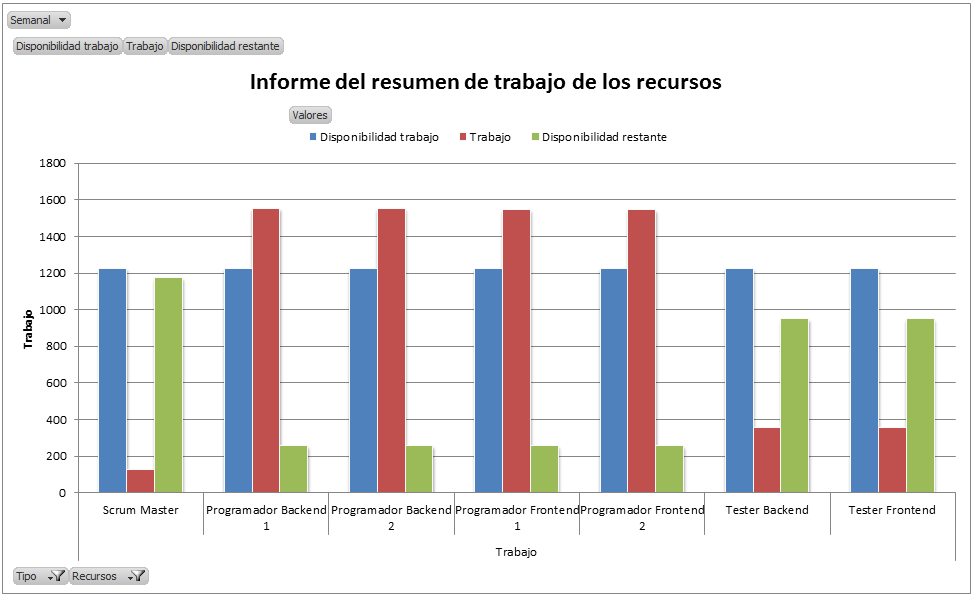
\includegraphics[width=0.8\textwidth]{img/tp2_capitulo3/resumen-trabajo-recursos}
    \caption{Informe del resumen de trabajo de los recursos.}
    \label{resumen-trabajo-recursos}
\end{figure}

\section{Análisis de factibilidad}

El análisis de factibilidad forma parte del proceso de evaluación al cual debe someterse nuestro proyecto.
Para abordar este tema, enfocaremos nuestros esfuerzos en distintas áreas que comprenden el análisis completo de factibilidad. %FUENTE: http://www.gestiopolis.com/estudio-integral-de-factibilidad-de-proyectos-de-inversion/
A partir de dicha cuestión, se evaluarán las siguientes factibilidades: técnica, operativa, financiera, legal y ambiental.

Al momento de realizar estas evaluaciones, se tiene en cuenta que en el contexto global los registros médicos personales, \textit{PHR} por sus siglas en inglés, son sistemas en crecimiento que tienen menos de media década los más antiguos.
Esto no es llamativo, ya que podemos observar que de los sistemas que existen actualmente, no hay ninguno que lleve la delantera sobre el resto.
%fuente https://en.wikipedia.org/wiki/Personal_health_record


\subsection{Factibilidad técnica}

\subsubsection{Introducción}

Indica si se dispone de los conocimientos y habilidades en el manejo de métodos, procedimientos y funciones requeridas para el desarrollo e implantación del proyecto.
Además indica si se dispone del equipo y herramientas para llevarlo a cabo, y de no ser así, si existe la posibilidad de generarlos o crearlos en el tiempo requerido por el proyecto. %FUENTE : https://es.wikipedia.org/wiki/Factibilidad#Factibilidad_t.C3.A9cnica_o_tecnol.C3.B3gica

\subsubsection{Aspectos de interés}

En los siguientes apartados se desarrollan los aspectos de interés de mayor relevancia que han sido analizados, atendiendo al carácter técnico de la factibilidad del proyecto.
Estos se pueden clasificar en las siguientes categorías:

\begin{itemize}
    \item Nivel de automatización de las funciones.
    \item Tipos de captura de datos.
    \item Sistema de respaldo.
    \item Seguridad.
    \item Integración con otros sistemas y otras TI, internas y externas.
\end{itemize}


% \item Volumen de datos, tipos de datos.
% \item Tipo de procesamiento de datos.

\subsubsection{Nivel de automatización de las funciones}
    
    La etapa de prueba del proyecto, en cada uno de los \textit{sprints}, se encuentra completamente automatizada mediante el servicio de \textbf{integración continua}.
    La integración continua permite que se ejecuten todos los casos de prueba de la aplicación, incluyendo pruebas unitarias y de integración, cada vez que se realizan cambios en la implementación del sistema.
    De esta manera, y mediante la creación de casos de prueba valiosos y de interés para el sistema, se pueden detectar a tiempo no sólo errores de implementación de las nuevas funcionalidades, sino también errores de regresión por cambios que generan defectos en la implementación que hasta el momento funcionaba correctamente.
    
    La etapa de despliegue del proyecto también será completamente automatizada, mediante un sistema de \textbf{despliegue continuo}.
    El despliegue continuo permite que el sistema sea desplegado cada vez que se realizan cambios en el mismo, y una vez que el sistema de integración continua determina que se cumplen con éxito todos los casos de prueba.
    
    Por lo tanto, serán necesarios tres servidores a ser utilizados durante todo el ciclo de vida del proyecto: un servidor de integración continua y dos servidores de hosting y despliegue continuo, uno para la capa de servicio (API) del sistema, y uno para la capa de presentación web.
    
    Las especificaciones recomendadas necesarias para cada uno de estos servidores se detallan a continuación, en los \textbf{Cuadros \ref{especificaciones-servidor-integracion-continua}}, \textbf{\ref{especificaciones-servidor-hosting-frontend}} y \textbf{\ref{especificaciones-servidor-hosting-backend}}.
    
    \begin{table}[h]
        \centering
        \begin{tabular}{|l|c|}
            \hline
            \multicolumn{2}{|c|}{{\bf Servidor de integración continua}}                  \\ \hline
            {\bf Procesador}                  & Doble núcleo, a 2 GHz                     \\ \hline
            {\bf Memoria RAM}                 & 2 GB                                      \\ \hline
            {\bf Capacidad de almacenamiento} & 500 GB                                    \\ \hline
            {\bf Ancho de banda}              & 1 Mbps                                    \\ \hline
            {\bf Sistema operativo}           & Ubuntu Server 14.04 LTS, arquitectura x64 \\ \hline
        \end{tabular}
        \caption{Especificaciones del servidor de integración continua.}
        \label{especificaciones-servidor-integracion-continua}
    \end{table}
    
    \begin{table}[h]
        \centering
        \begin{tabular}{|l|c|}
            \hline
            \multicolumn{2}{|c|}{{\bf Servidor de hosting y despliegue de capa de servicio}} \\ \hline
            {\bf Procesador}                  & Cuatro núcleos, a 3 GHz                      \\ \hline
            {\bf Memoria RAM}                 & 8 GB                                         \\ \hline
            {\bf Capacidad de almacenamiento} & 500 GB                                       \\ \hline
            {\bf Ancho de banda}              & 100 Mbps                                     \\ \hline
            {\bf Sistema operativo}           & Ubuntu Server 14.04 LTS, arquitectura x64    \\ \hline
        \end{tabular}
        \caption{Especificaciones del servidor de hosting y despliegue de capa de servicio.}
        \label{especificaciones-servidor-hosting-frontend}
    \end{table}
    
    \begin{table}[h]
        \centering
        \begin{tabular}{|l|c|}
            \hline
            \multicolumn{2}{|c|}{{\bf Servidor de hosting y despliegue de capa de presentación web}} \\ \hline
            {\bf Procesador}                  & Doble núcleo, a 3 GHz                                \\ \hline
            {\bf Memoria RAM}                 & 8 GB                                                 \\ \hline
            {\bf Capacidad de almacenamiento} & 150 GB                                               \\ \hline
            {\bf Ancho de banda}              & 30 Mbps                                              \\ \hline
            {\bf Sistema operativo}           & Ubuntu Server 14.04 LTS, arquitectura x64            \\ \hline
        \end{tabular}
        \caption{Especificaciones del servidor de integración continua.}
        \label{especificaciones-servidor-hosting-backend}
    \end{table}
    
    
\subsubsection{Tipos de captura de datos}:
    
    El sistema permitirá tres tipos de captura de datos, para facilitar la carga de datos no sólo por parte de pacientes sino también de médicos, especialistas de salud y cualquier usuario autorizado por el mismo para ingresar datos en su perfil:
    
    \begin{enumerate}
        \item Ingreso manual de estudios médicos y mediciones.
        \item Carga automatizada por parte de sistemas externos, a través de servicios expuestos por el propio sistema en su API pública.
        \item Ingreso de datos automatizado mediante reconocimiento óptico de caracteres (\textit{OCR}), a partir de documentos fotografiados. 
    \end{enumerate}
    
    Cada uno de estos tipos de captura de datos implica tomar en consideración diferentes aspectos técnicos y operativos.
    
    En el caso del \textbf{ingreso manual}, se debe proveer al usuario final de interfaces de usuario intuitivas.
    Para esto, se hará uso de \textbf{AngularJS}, un \textit{framework web} orientado a la creación de interfaces de usuario.

    En el caso de la \textbf{carga automatizada por parte de sistemas externos}, se logrará mediante la incorporación e implementación de estándares.
    Específicamente, la estructuración del sistema considerando la documentación de los \textbf{estándares médicos HL7 y DICOM}, orientados a la estandarización de los procesos de comunicación, almacenamiento, transferencia y representación de información médica, facilitará la interacción del sistema con sistemas externos ubicados en hospitales y centros de salud, como así también la comunicación entre usuarios del propio sistema.
    
    Para el caso del \textbf{ingreso automatizado de datos médicos} por parte del usuario final, la funcionalidad depende exclusivamente de aplicaciones y librerías que provean el reconocimiento óptico de caracteres, llamado \textbf{OCR} (\textit{Optical Character Recognition}).
    Si bien es un área en la que hace falta un avance considerable para que los resultados sean completamente confiables, el grado de confianza con los resultados a partir de documentos médicos, los cuales generalmente incluyen una estructura de documento simple y limitaciones en cuanto a su extensión, es muy alto y permiten la inclusión de esta funcionalidad en el sistema.
    

% \item Frecuencia y volumen de ingreso de datos.
% \item Frecuencia, formas, soporte y volumen de información a generar.
% \item Formularios.
% \item Funcionamiento ininterrumpido de sistemas, utilización de equipos, horarios.
% \item Método de desarrollo, testing, capacitación, implementación y mantenimiento.


\subsubsection{Sistema de respaldo}
    
    El sistema de respaldo de datos debe considerar la importancia y sensibilidad de los datos que maneja y almacena el sistema, que son de vital importancia para el dueño de la información, y para los encargados de velar por su salud.
    No es aceptable la pérdida de información, por lo que se hace uso de la siguiente política de respaldo:
    
    \begin{itemize}
        \item \textbf{Respaldos completos}:
        A ser realizados semanalmente, en soporte de cinta magnética y almacenados fuera del edificio principal, en caja de seguridad ignífuga.
        
        \item \textbf{Respaldos incrementales}:
        A ser realizados diariamente, en discos rígidos de servidores, provistos especialmente para razones de respaldo incremental. 
    \end{itemize}
    
    No se hace uso de servicios de respaldo en la nube provistos por empresas ajenas, debido a la confidencialidad de los datos que maneja el sistema.
    Esto es debido a que, incluso con una encriptación fuerte de los datos a ser almacenados en tales servidores, no hay garantías de que los sistemas de software de las compañías contratadas no incluyen \textit{puertas traseras} o vulnerabilidades que hagan accesible la información antes de que ésta sea encriptada.
    
    Además, se tiene en cuenta que, si bien actualmente una clave de gran tamaño para la encriptación puede ser lo suficientemente segura, con el pasar del tiempo y el aumento de la tecnología se consigue descifrar mediante fuerza bruta datos cifrados con claves cada vez más grandes.
    Esto, sumado a que no se tiene certeza de cuánto tiempo es el que realmente almacenan los datos las compañías externas, permite concluir que no es conveniente confiar en el servicio de respaldo, incluso encriptado, por parte de terceros.
    
    
% \item Infraestructura e instalaciones.


\subsubsection{Seguridad}
    
    Debido a la confidencialidad y la sensibilidad de los datos de los que se vale el sistema, es fundamental mantenerlos en forma segura y privada, para que no pueda ser accedida por personas o empresas malintencionadas para hacer uso de ellos basándose en sus propios intereses.
    
    Además, es importante considerar que, básicamente, todo estudio médico o información de salud de la persona representa un aspecto crítico e, incluso, una debilidad o falencia en su salud.
    Esto puede afectar negativamente en los aspectos interpersonales, laborales, económicos e incluso intrapersonales, y por lo tanto es necesaria la mayor discreción y confidencialidad posible de la información.
    
    La solución desde el punto de vista técnico para mantener a salvo la información de la persona, es el \textbf{cifrado} de todos los datos y documentos de la misma.
    
    El algoritmo \textbf{AES} (\textit{Advanced Encryption Standard}) es el sucesor del algoritmo DES como algoritmo estándar de encriptación simétrica, para los organismos federales de los Estados Unidos (y como estándar para la mayor parte del mundo, también).
    AES acepta claves de 128, 192 o 256 bits (128 bits es inviolable actualmente), usa bloques de 128 bits y es eficiente tanto por software como por hardware.
    Fue seleccionado a través de una competencia abierta en la que participaron cientos de criptógrafos durante varios años.
    
    AES es un algoritmo de cifrado simétrico.
    Esto significa que tanto el cifrado como el descifrado de la información se lleva a cabo utilizando la misma clave.
    Haciendo uso del algoritmo AES se logra el cifrado y la confidencialidad de la información almacenada en el sistema.
    
    Sin embargo, otra consideración y preocupación por parte de los usuarios es que sus datos, aún cifrados, puedan ser accedidos por personal interno a nuestra organización, al tener posesión de las claves utilizadas.
    
    Es por esto, que el enfoque a utilizar es similar al del popular sitio de almacenamiento cifrado \textbf{Mega}, al realizar el encriptado.
    Así, la información y documentos médicos son encriptados del lado del cliente mediante el uso del algoritmo AES y luego transferidos al sistema.
    El desencriptado también se hace del lado del cliente, mediante la utilización de la misma clave.
    
    De esta forma, la organización no conoce ni almacena las llaves de encriptación, por lo que no tiene forma de acceder a la información personal y sensible de sus usuarios.
    

% \item Recuperación.


\subsubsection{Integración con otros sistemas}
    
    La \textbf{arquitectura} del sistema, basada en una API e interfaces de usuario que se comunican con la misma, unido a la implementación y la estructuración en base a los estándares \textbf{HL7} y \textbf{DICOM}, permiten la completa integración con otros sistemas de salud que manejen estos estándares.
    
    Los \textbf{sistemas que aportan valor} al generar comunicaciones que solicitan o proveen datos, son aquellos sistemas alojados en hospitales, centros médicos y toda otra institución de salud.
    
    El \textbf{objetivo} al proveer una API que cumpla con las directrices y especificaciones de los estándares mencionados anteriormente, es el facilitar la comunicación a mediano y largo plazo con estos sistemas, llegando a ser así el nexo fundamental entre sistemas de salud de diferentes instituciones.
    Pero, al mismo tiempo, no depender completamente de los estas instituciones, al permitir el uso y la carga de información por parte de usuarios finales o de sus médicos, mediante las interfaces de usuario provistas, que aprovechan la arquitectura de capas del sistema.
    
    
% \item Crecimiento estimado en la empresa que afecte al Sistema.
% \item Crecimiento funcional y de TI para el Sistema.
% \item Flexibilidad para nuevas TI.


\subsubsection{Conclusión}

Atendiendo a la arquitectura propuesta y a las funcionalidades que caracterizan al sistema, se establece que las tecnologías para llevarlo a cabo existen y se encuentran disponibles libremente.

Además, considerando como aspecto fundamental la seguridad y confidencialidad de los datos de los que el sistema se vale y almacena, y previendo el uso de algoritmos de encriptación en conjunto con sistemas locales de respaldo, se concluye que el proyecto es \textbf{técnicamente factible}.


\subsection{Factibilidad operativa}

\subsubsection{Introducción}

Se refiere a que debe existir el personal capacitado requerido para llevar a cabo el proyecto y así mismo, deben existir usuarios finales dispuestos a emplear los productos o servicios generados por el proyecto o sistema desarrollado. %FUENTE : http://es.wikipedia.org/wiki/Factibilidad#Factibilidad_humana_u_operacional

\subsubsection{Aspectos de interés}

% Algunos aspectos que debemos analizar son:
% \begin{itemize}
% \item Personas (PPPP), personal permanente, temporario, 
% asesoramiento.
% \item Diseño de campaña para involucrar a los usuarios.
% \item Capacitación.
% \item Apoyo gerencial.
% \item Aceptación de entregables por parte de usuarios.
% \item Testing con usuarios.
% \item Motivación, rendimiento, cumplimiento, rechazo al 
% Sistema.
% \item Insumos, servicios de apoyo.
% \item Relación con otras áreas.
% \item Normas y procedimientos propios del Sistema y de la empresa.
% \item Momento de implementación, estabilización y aceptación del Sistema.
% \item Planificación, organización, dirección.
% \item Trabajo en equipos efectivos.
% \item Resolución de conflictos.
% \item Técnicas de gestión de RRHH.
% \item Actividades relacionadas con conversión del Sistema, control y seguimiento
% \end{itemize}


El sistema planteado se focaliza en resolver una necesidad pública y general, donde nuestros usuarios serán personas que deseen otorgarle una organización y una mejor administración a la gestión de la información de salud personal, como así también a los médicos que deseen participar activamente comentando y realizando solicitudes a sus pacientes a través de la plataforma.
Por este tipo de usuarios, nos enfrentamos a un problema particular, que es el no alcanzar la cantidad de usuarios esperados.

Analizando esto, se ha encuadrado el análisis de factibilidad operativa en los siguientes aspectos:

\begin{itemize}
    \item Conocimiento de la existencia del software por parte del público en general y su utilidad.
    \item Facilidad de carga de información.
    \item Facilidad de uso del sistema.
    \item Garantía de seguridad en la gestión de datos.
    \item Manejo y resolución de conflictos.
    \item Conversión del sistema.
\end{itemize}


\subsubsection{Conocimiento de la existencia del software}
\label{conocimiento_del_software}
    
	Este aspecto implica el conocimiento, por parte del público, de la existencia del software y su utilidad.
    Será abordado a través de la asistencia de un profesional de Marketing, el cual asistirá a la organización en cuestiones relacionadas al posicionamiento y publicidad de nuestros servicios.
    
    Como primera impresión, podemos dirigir nuestros esfuerzos en dos direcciones:
    
    \begin{itemize}
        \item Primero, hacia el paciente.
        Éste, siendo consciente o hasta sin saberlo, desea mejorar su manera de gestionar los análisis médicos o el seguimiento de su información de salud.
        \item Y segundo, hacia los profesionales de la salud que deseen mejorar su eficiencia y calidad en diagnósticos médicos.
    \end{itemize}
    
    Se invertirá en realizar publicidad en aquellos sitios web de salud que lo permitan, para atraer a aquellos usuarios interesados por su cuidado personal.
    
    Además, se utilizarán lugares relacionados a la salud, para dar a conocer nuestro producto.
    Estos lugares pueden ser hospitales, farmacias, centros de salud y cualquier otro tipo de institución de salud.
    Se aprovechará la intima relación que tiene el sistema con los lugares antes citados para establecer convenios que permitan el beneficio mutuo, a partir de la prestación del servicio del propio sistema. 
    
    Por ejemplo, actualmente existen farmacias que brindan a sus clientes, la posibilidad de acceder a una cuenta para ver los productos que se ha comprado a lo largo de su historia como cliente, dándoles puntos por cada compra que luego podrán canjear.
    Sería interesante ofrecer el sistema a esas farmacias, para que ellos le brinden a sus clientes más beneficios, y así el sistema se beneficiaría con la popularidad del mismo.
    
	La reputación que se vaya logrando generará una necesidad en el ámbito médico gerencial, de manera que, al notar las ventajas provistas por la plataforma, se promoverá entre sus médicos dependientes la utilización del mismo.
    A lo anterior debemos añadir la influencia que reciban por parte de los pacientes, que provean su información cargada en el sistema.
    
    Sin embargo, se tendrá en cuenta la posibilidad de que los hospitales nieguen la participación de sus médicos en el uso del sistema, privando de información relevante para la toma de decisiones sobre la salud de los pacientes.
    Esto podría suceder porque el hospital tenga un sistema propio y no quiera alentar a su abandono. 
    
    Teniendo en cuenta lo anterior, el sistema desarrollado presenta una capa de servicios que con mínimos cambios en los sistemas actuales permitiría la existencia e interacción de ambos.
    En ultima instancia, se permitirá enviar por correo electrónico gráficas de mediciones o análisis médicos , o su impresión.

    Además, el profesional de Marketing, ayudará a definir determinados hitos del proyecto, como por ejemplo en que momento ir liberando al público nuestros servicios.
    
    
\subsubsection{Facilidad de carga de información}
    
    Consideramos esta característica, fundamental de resolver.
    Esto es debido a que, al observar los sistemas actuales, no sólo encontramos que es un aspecto de riesgo sino también que el resolverla sería muy ventajoso para el proyecto. 
    Al modularizar, para mantener un bajo acoplamiento entre las tecnologías de Front-end y la capa de servicios, ofrecemos un servicio flexible en tecnologías de vista para el usuario, lo que consideramos de extrema importancia, ya que nos encontramos en un momento donde los smartphones están ampliamente establecidos en el mercado, pero también hay otras tecnologías fuertemente emergentes, como los dispositivos wearables.
    
    La capa de servicios permite que se puedan conectar directamente ciertos dispositivos personales, que se encargan de tomar mediciones relacionadas a la salud.
    También permite que el hospital que lo desee, haga uso directamente del sistema, con una interfaz propia para sus pacientes.
    

\subsubsection{Facilidad de uso del sistema}
    
    Las tecnologías seleccionadas para el Front-end aplican directamente a este ítem.
    Se hace uso de \textbf{AngularJS}, para brindarle al usuario una experiencia completamente interactiva; \textit{frameworks} de vista como \textbf{Bootstrap}, que le da una sensación de frescura a la web y lo mantiene con una distribución de íconos familiar.
    Es importante recalcar que éste es uno de los \textit{frameworks} más utilizados.
    
    También, las capacitaciones fueron específicamente elegidas teniendo cuenta el desarrollo de un producto fácil, integral e intuitivo para los usuarios finales al apoyarse, entre otros recursos, en recomendaciones de los experimentados y consolidados diseñadores de \textbf{HackDesign.org}.
    
    Cabe destacar que el sistema estará \textbf{centrado en el usuario}.
    Esto se caracteriza por asumir que todo el proceso de diseño y desarrollo, tanto del sitio web como plataformas de acceso móvil, deben estar conducidas por el usuario, sus necesidades, características y objetivos.

	Centrar el diseño de la interfaz en los usuarios implica:
	\begin{itemize}
		\item Involucrar desde el comienzo a los usuarios.
		\item Conocer cómo son.
		\item Saber qué necesitan.
		\item Investigar cómo reaccionan ante el diseño.
		\item Cómo es su experiencia de uso.
		\item Innovar siempre con el objetivo claro de mejorar la experiencia del usuario.
	\end{itemize}
	Para fortalecer y garantizar los ítems anteriormente analizados, se realizarán pruebas con personas voluntarias durante distintas etapas del desarrollo del proyecto.%En base al test de usabilidad que se adjunta en el anexo XX
%Anexar prueba : http://intergraphicdesigns.com/tools/test-usabilidad-web


\subsubsection{Garantía de seguridad en la gestión de datos}
    
    Internet ofrece muchas oportunidades para explorar, crear y colaborar.
    Y para aprovechar la Web al máximo, es importante mantener al usuario protegido y seguro.
    Por lo cual, el sistema hará uso y estará fundado sobre los siguientes conceptos:
    
    \begin{itemize}
    	\item \textbf{Certificado digital}:
    
		Un certificado digital es una credencial electrónica que puede usarse para establecer la identidad de un usuario, en cualquier lugar en que se encuentre ese usuario.
    	Al igual que un documento de identidad, como una licencia de conducir, un certificado digital debe tener ciertas características para que se lo pueda utilizar como una forma de identificación.
	    Concretamente debe cumplir con lo siguiente:
    
		\begin{itemize}
    		\item Nombrar la cuenta específica que se identifica.
		    \item Ser emitido por una autoridad que pueda revocar el certificado en cualquier momento.
		    \item Ser difícil de falsificar.
	    	\item Contener un aval de la autoridad que lo emite; en este caso, nuestra organización.
		\end{itemize}
    
		\item \textbf{Autenticación}:
    
		Puesto que todos los usuarios del sistema poseerán credenciales digitales, cualquier usuario puede verificar la identidad de otro.
	    El proceso de comprobar la identidad de las partes se llama \textbf{autenticación}.
    	Para acceder al certificado digital, es necesario confirmar su nombre de usuario y contraseña.

		\item \textbf{Cifrado}:

		Las redes de comunicaciones, tales como Internet, pueden ser controladas por delincuentes y piratas informáticos en distintos puntos.
	    Ésta es una de las razones por las que el correo electrónico y muchos programas de mensajería instantánea en Internet se consideran poco fiables desde el punto de vista de la seguridad.
    	En otras palabras, dado que personas desconocidas disponen de muchas formas de controlar las comunicaciones de los usuarios, estos últimos deben tomar medidas para protegerse a sí mismos contra este tipo de intrusiones.

		El cifrado es el proceso de codificación de mensajes que usa principios de las matemáticas, de forma tal que solo el destinatario específico pueda leerlos.
		Durante siglos se desarrollaron muchos tipos de técnicas de cifrado, pero todas se parecen a una caja fuerte y una llave: una vez que un mensaje secreto se coloca en la caja fuerte y se asegura con la llave, sólo puede leerlo alguien que posea la misma llave. 
	    La llave puede ser algo conocido o un objeto físico; por ejemplo, el largo y el ancho del cilindro que mencionamos anteriormente.
        En el sistema, la llave será el nombre de usuario y contraseña.
        De allí la importancia de protegerlos.

		Se utilizarán algoritmos de cifrado basados en normas acreditadas para evitar que las comunicaciones de los usuarios caigan en manos de delincuentes y piratas informáticos. De esa manera, se ayuda a asegurar la privacidad del usuario y la integridad de los datos que un usuario le envía a otro.
    \end{itemize}
    

\subsubsection{Manejo y resolución de conflictos}

A continuación, se especifican una serie de conflictos que podrían presentarse durante la ejecución del proyecto:

\begin{itemize}

\item \textit{Un desarrollador inexperto no sabe cómo resolver un problema que requiere conocimientos de patrones de diseño de software}:

El director consulta al líder técnico, y éste demuestra gran capacidad para resolver el conflicto.
Luego, para evitar futuros conflictos y seguir el enfoque de colaboración, el director reúne al conjunto de desarrolladores inexpertos con el líder técnico y resuelven el conflicto de forma colaborativa y con el objetivo de aprender y evitar que el conflicto se repita en el futuro, manteniendo el aprendizaje en la base de conocimiento del equipo.

\item \textit{Un desarrollador resuelve un problema de diseño que no esté de acuerdo con consideraciones de cohesión y acoplamiento}:

Siguiendo un enfoque \textbf{agresivo}, podría aceptarse esta solución rápida y continuar con el desarrollo.
Sin embargo, según el enfoque de arreglo, esta solución genera inconsistencias o errores futuros, por lo que la decisión del director debería ser la de frenar la actividad de diseño y continuarla en conjunto con alguien que posea los conocimientos para resolver el problema de forma correcta en cuanto a estas cuestiones esenciales en la etapa de desarrollo.

\item \textit{El desarrollador no recibe suficiente descripción o claridad acerca de los defectos por parte del tester}:

Este conflicto genera que los arreglos que realiza el desarrollador pueden no llegar a ser los adecuados.
Por esto, se define una plantilla que debe seguir el tester, la cual funciona como respaldo cuando los pedidos de colaboración no dan resultado.

\item \textit{Pobre comunicación entre los participantes sin alguna razón aparente}:

El director tendrá que entrar en acción y lograr que se entienda que para la concreción del proyecto es importante que los integrantes se comuniquen más allá de sus diferencias, por sus propias personalidades o por cualquier tipo de conflicto que tengan entre ellos.
El director debe identificar estas situaciones y tomar un enfoque de \textbf{arreglo} y \textbf{agresivo}, en el que va a dar las instrucciones y guiará la comunicación sin olvidar de seguir cada uno de los acontecimientos.

\item \textit{Uno de los participantes no realiza su parte del trabajo}:

Puede ocurrir que por diversos motivos (personal, laboral u otros), uno de los participantes del proyecto no esté llevando adelante las tareas que le corresponden.
En este tipo de casos, el director deberá intervenir tomando un enfoque de \textbf{colaboración}, preguntando qué sucede, por qué no realizó el trabajo asignado, tratando de solucionar posibles conflictos y poniéndose a disposición de sus liderados.

\item \textit{Reuniones poco eficaces}:

Ocurre muchas veces, que en las reuniones de trabajo no se avanza tanto como se espera.
Esto puede ser por distracción, no muy buena planificación de las tareas y tiempos que llevará cada una.
En estos casos, el director deberá estructurar las reuniones de forma tal que no deje lugar a la distracción y se aproveche en un 100\% el tiempo para las actividades que deben ser previamente planificadas.
Se recomienda que el director actúe preguntando a cada miembro qué se puede hacer, qué actividades se pueden llevar adelante y los tiempos estimados para las mismas.
También es de utilidad definir moderadores que cambien con el tiempo y apoyen en el objetivo de hacer reuniones útiles tanto para los participantes como para el proyecto.

\item \textit{Poca motivación de los miembros}:

Puede ocurrir que algunos miembros del grupo se encuentren desanimados.
Esto puede deberse a situaciones personales; puede que no estén a gusto con la actividad que realizan o con el mismo proyecto.
El director puede asumir un enfoque de \textbf{colaboración} y percibir las inquietudes, proponer mejoras motivacionales para llegar a un consenso y obtener así compromiso de parte de los participantes, haciéndolos sentir una parte fundamental del equipo.

\item \textit{Falta de conocimientos del equipo}:

Este es el caso en el que algunos integrantes dominen, mejor que otros, determinadas herramientas, o demuestren mayores capacidades para resolver tareas en menos tiempo y con mejores resultados.
Esto puede generar inconvenientes porque algunos trabajan más y obtienen mayor cantidad de resultados que otros.
En este tipo de casos, el líder del equipo debe tomar un enfoque \textbf{colaborativo}, capacitando a aquellos que lo requieran, y de \textbf{arreglo}, al brindar beneficios a aquellos con conocimientos y que dediquen tiempo a compartir y enseñar a los demás.
El director debe dar apoyo, acompañamiento y disolver los sentimientos que han interferido en la relación de los participantes.

\end{itemize}


\subsubsection{Conversión del sistema}

Dado que la conversión del sistema es esencial para una correcta adopción por parte de los usuarios del mismo, se consensuará entre el equipo y su Director de Proyecto cuál será el método de conversión del Sistema (para pasar del sistema actual al nuevo), con todas las actividades a realizar.
Se registrará en este punto no sólo el método y las actividades sino también la justificación correspondiente.

Antes de continuar, se debe aclarar que no se pretende eliminar el sistema de historia clínica que actualmente usan los centros de salud, pero si se encuentra en nuestros planes que las personas puedan utilizar este sistema como medio de comunicación con el médico.

Se es consciente que lograr que los pacientes utilicen el sistema será un gran desafío, pero para esto se armará un plan de conversión estratégico detallando los métodos y actividades necesarios para la conversión junto con la justificación correspondiente.

Actualmente, existen 5 métodos de conversión de sistema:
\begin{itemize}
    \item Conversión directa.
    \item Conversión paralela.
    \item Conversión gradual o por fases.
    \item Conversión de prototipo modular.
    \item Conversión distribuida.
\end{itemize}

En el proyecto, se utilizará el método de \textbf{conversión paralela}, ya que el sistema convivirá con la forma de gestión que posea el usuario, permitiéndole la posibilidad  de comparar las ventajas y detectar los beneficios que brinda el nuevo sistema.
Además, este método está recomendado para aquellos casos en los que un sistema computarizado remplaza uno manual y es lo que se pretende hacer en el proyecto.

A continuación, se describirán todas las actividades que se llevarán a cabo para implementar el nuevo sistema.
Se identificará a todas las personas responsables de cada actividad y el tiempo correspondiente a cada una.


\begin{enumerate}
\item \textbf{Preparación de datos y archivos}:

Será necesario determinar cuál será la base de conocimiento que se cargará en el sistema; éstas deberán cumplir con los estándares medicinales, y algunos ejemplos son:

\begin{itemize}
    \item Especialidades.
    \item Tipos de  análisis.
    \item Tipo de mediciones .
    \item Formatos de análisis.
    \item Sobre el paciente: sexo, enfermedades, estados fisiológicos, etc.
    \item Información farmacológica: alergias, medicamentos.
    \item Productos comerciales: productos farmacéuticos que se comercializan en un área o región, nombre comercial, presentación, dosificación, precio, cobertura, tipo de dispensación, conservación, origen, laboratorio que lo produce.
    Las fuentes de donde se obtiene la información son la industria farmacéutica, financiadores de salud y farmacólogos clínicos.
    Estos datos son generalmente mantenidos por empresas abocadas a tal fin y en algunos casos por organismos oficiales encargadas de informar periódicamente a sus suscriptores sobre las altas, bajas o modificaciones de productos medicinales.
    \item Principios activos o monodrogas: nombre genérico, sinónimos, clasificación farmacológica y/o terapéutica, farmacodinamia y farmacocinética, preparación, formas de administración, rango de dosis recomendada, dosificación en pacientes pediátricos, dosificación en ancianos, dosificación en insuficiencia renal, dosificación en insuficiencia hepática severa, dosificación en cirrosis, embarazo y lactancia, sobredosis, precauciones, indicaciones, contraindicaciones, reacciones adversas, antagonismos y antidotismos, interacciones, efectos sobre exámenes de diagnóstico e información para los pacientes.
    \item Terminología médica: Unified Medical Language System (UMLS); SNOMED CT terminología clínica integral, multilingüe y codificada de mayor amplitud, precisión e importancia desarrollada en el mundo; variantes léxicas, opciones controladas, reglas terminológicas, CIAP-2 Clasificación Internacional de Atención Primaria.
    \item Prestadoras, aseguradoras, lugares físicos y prestaciones.
\end{itemize}

Además, se deberá modelar el sistema para que permita futuras conexiones con otros similares ya existentes, como pueden ser de laboratorios o la historia clínica del hospital al que incurre el paciente que quiere utilizar el sistema.
Una solución a este posible conflicto es el ofrecer una API que permita la conexión de sistemas ajenos al nuestro.

\item \textbf{Configuración y diseño del sistema}:

Para facilitarle el acceso al usuario se implementará el sistema en una plataforma web utilizando un servidor diferente del servidor que gestionará las conexiones a la API y a la base de datos.

Esta arquitectura será mejor a la hora de escalar, para soportar y brindar servicio a los usuarios que lo requieran, sin incurrir en tiempos prolongados de espera ni modificaciones en la arquitectura y el diseño del sistema.


\item \textbf{Capacitación e instrucciones de uso}:

El usuario alcanzará una mejor, y más completa experiencia de uso, haciendo uso de herramientas de aprendizaje, que serán de apoyo a las funciones regulares ofrecidas.
Estas herramientas son:
	\begin{itemize}
		\item Tutoriales visuales, se añadirán mensajes de ayuda en la misma vista que permita al usuario comprender todas y cada una de las opciones. Esto se implementara con un asistente de iniciación interactiva que le permite al usuario que ingresa por primera vez conocer cuales son las funcionalidades que brinda el sistema.
		\item Se ofrecerán videos para explicar el funcionamiento del sistema desde el punto de vista del paciente y del médico en alguna plataforma de reproducción online, como Youtube, para las personas que necesiten de otras alternativas.
        \item Se contará con botones de ayuda en los distintas herramientas provistas por el sistema,para que el usuario pueda encontrar rápidamente lo que está buscando y explotar la máximo las funcionalidades otorgadas.

        \item El manual de usuario, que incluirá las siguientes secciones:
        \begin{itemize}
            \item   Una página de portada.
            \item   Una página de título.
            \item   Una página de derechos de autor.
            \item   Un prefacio, que contiene detalles de los documentos relacionados y la información sobre cómo navegar por la guía del usuario.
            \item   Una página de contenido.
            \item   Una guía sobre cómo utilizar al menos las principales funciones del sistema, es decir, sus funciones básicas.
            \item   Una sección de solución de problemas que detalla los posibles errores o problemas que pueden surgir, junto con la forma de solucionarlos.
            \item   Una sección de preguntas frecuentes.
            \item   Dónde encontrar más ayuda, y datos de contacto.
            \item   Un Glosario y, para documentos más grandes, un Índice.
        \end{itemize}
	\end{itemize}

\item \textbf{Publicidad y propaganda}:

Este item ya fue desarrollado, en la \textbf{Sección \ref{conocimiento_del_software}}.


\subsubsection{Otras consideraciones}

	Hay aspectos de análisis que no se pueden encuadrar en los ítems anteriores.
    Sin embargo afectarían al desenvolvimiento operativo del sistema.
    Entre ellos, encontramos los siguientes:
    
    \textbf{Relación con otras áreas}: una adopción general del sistema podría implicar un interés de otros sectores sobre el sistema:
    
    \begin{itemize}
        \item Hospitales: el sistema impactará directamente en ellos, ya que los médicos utilizaran la información que los pacientes les provean a través de nuestro sistema.
        \item Industria farmacéutica: podría necesitar consumir información estadística recopilada por el sistema por ejemplo para saber cuando lanzar un producto al mercado
        \item Laboratorios de análisis clínicos: podría el sistema significar una nueva forma de devolver resultados de análisis a sus clientes, impactando en la forma de realizar sus actividades.
        \item Gobierno: podría necesitar consumir información del sistema para la planificación de estrategias de salud pública o también podría impactar en las leyes de información de salud vigentes.
    \end{itemize}

    \textbf{Personal adicional}: las personas que participarán en el sistema y que no forman parte del equipo de desarrollo directamente, serán:

 \begin{itemize}
     \item Licenciado en Comercialización (Marketing): se encargará de gestionar las actividades relacionadas al posicionamiento del proyecto a nivel de negocios, y será fundamental para amoldar el producto a las necesidades del consumidor, como así también para generar las propuestas de valor para satisfacer las mismas y preparar a la empresa para enfrentar con éxito a los consumidores.
	\item Usuarios generales voluntarios: que probarán la usabilidad de las interfaces.
    \item Médicos probadores: evaluarán la interfaz de usuario del sistema para los profesionales de la salud.
    También, realizarán criticas constructivas sobre la estructura, para así poder desarrollar un sistema que les provea mayor y mejor información en el soporte de sus decisiones.
    \item Médicos asesores: son contactos dentro de la medicina que ofrecen una visión desde dentro del marco de la salud, ante dudas relacionadas tanto al relevamiento de la información que formará parte de la estructura del sistema, como enfermedades, medicamentos o tipos de análisis clínicos.
    \item Diseñador gráfico: el mismo participará en el proyecto con una función de soporte sobre el diseño de interfaz y para realizar cuestiones gráfica fuera del alcance de los desarrolladores.
    \item Abogado: formará parte de algunas reuniones de diseño, sobre todo para aclarar cuestiones legales sobre el manejo de información sensible.
\end{itemize}


\end{enumerate}

\subsubsection{Conclusión}

Como se desarrolló previamente, debemos atender a cuestiones como lograr hacer conocer el sistema en el público en general y, principalmente, en las personas que frecuentan hospitales o centros de salud.
Al mismo tiempo, ofrecer un servicio donde se priorice la facilidad de carga de datos y la seguridad de los mismos para no impactar negativamente en la imagen del sistema.

No debemos dejar de considerar cómo el sistema afecta a otras áreas, siendo éstas, quizás, fuentes importantes de ingresos en un futuro para nuestra organización, o siendo que también pueden impactar negativamente en el proyecto.

El hecho de que el sistema no sea para otra empresa, no facilita el aspecto operativo.
Sin embargo, tomando recaudos tales como el apoyarse sobre las herramientas correctas, previendo posibles riesgos futuros, la interacción continua con los usuarios y atendiendo a las relaciones del sistema con otras áreas, se puede concluir que el sistema es \textbf{operativamente factible}.


\subsection{Factibilidad legal}

\subsubsection{Introducción}

La privacidad y seguridad de la información están en las agendas legislativas de muchos países. Las regulaciones legales surgen en forma de leyes, actas, artículos constitucionales, entre otros, e imponen responsabilidades a las instituciones que almacenan información personal y otorgan derechos a los individuos. En algunos países hay regulaciones específicas para la información en salud, y en otros países hay regulaciones generales donde la salud está incluida. Los datos sobre la salud de los individuos están considerados dentro de los más ``sensibles'', o los de mayor impacto si se vulnera su privacidad.

En latinoamericana y específicamente en Argentina, los mecanismos de protección de datos se inspiran en la legislación europea, la cual usa la directiva 95/46/EC sobre la protección de datos personales.


\subsubsection{Aspectos de interés}

Los aspectos de interés de mayor relevancia legal que han sido analizados y se exponen en los siguientes apartados, brindando así el contexto legal del sistema, son los siguientes:

\begin{itemize}
    \item Leyes, resoluciones y normas vigentes.
    \item Jurisprudencia y casos similares relevados.
    \item Autorizaciones y habilitaciones de funcionamiento.
    \item Revisión de las acciones automáticas del sistema.
    \item Invasión de privacidad.
    \item Licenciamiento de software.
    \item Ataques externos, mediante Internet.
    \item Registración de marca.
    \item Incorporación de personal.
    \item Ley de industria del software.
    \item Subsidios y posibilidades de financiamiento.
\end{itemize}


\subsubsection{Leyes, resoluciones y normas vigentes}
    
    Un concepto común en el país es que las regulaciones se basen en el \textit{``Habeas Data''}.
    Esta frase se traduce literalmente del latín como ``tienes derecho a tus datos'':
    Es el principio por el cual todo individuo tiene derecho a conocer qué datos personales están siendo almacenados por terceros, y a actualizarlos, modificarlos, o incluso borrarlos.
    La implementación de este derecho implica la necesidad de registrar las bases de datos que contengan datos personales y designar responsables de cada una.
    
    A continuación, se listan las distintas leyes, normas y resoluciones vigentes, asociadas al manejo de información personal y, específicamente, a la información de salud:
    
	\begin{enumerate}
		\item \textbf{Constitución Nacional 1994} (Art. 43), citamos el párrafo 3:
        Toda persona podrá interponer esta acción para tomar conocimiento de los datos a ella referidos y de su finalidad, que consten en registros o bancos de datos públicos, o los privados destinados a proveer informes, y en caso de falsedad o discriminación, para exigir la supresión, rectificación, confidencialidad o actualización de aquellos.
        No podrá afectarse el secreto de las fuentes de información periodística.
		%Fuente http://pdba.georgetown.edu/Constitutions/Argentina/argen94.html
        \item \textbf{Ley 25.326}:
        Disposiciones Generales. Principios generales relativos a la protección de datos. Derechos de los titulares de datos. Usuarios y responsables de archivos, registros y bancos de datos. Control. Sanciones. Acción de protección de los datos personales.
        
        \begin{itemize}
			\item \textbf{Artículo 2º}: Definiciones de Datos personales; datos sensibles; archivo, registro, base o banco de datos; tratamiento de datos; responsable de archivo, registro, base o banco de datos; datos informatizados, titular de los datos; usuario de datos y disociación de datos. Cómo vemos son de especial importancia para nuestro sistema las definiciones de datos sensibles y responsable de archivo, registro, base o banco de datos.
            \item \textbf{Artículo 7º}: Ninguna persona puede ser obligada a proporcionar datos sensibles, los datos sensibles sólo pueden ser recolectados y objeto de tratamiento cuando medien
razones de interés general autorizadas por ley, también podrán ser tratados con finalidades estadísticas o científicas cuando no puedan ser identificados sus titulares y queda prohibida la formación de archivos, bancos o registros que almacenen información que directa o indirectamente datos sensibles.
			\item \textbf{Artículo 9º}: Hace referencia a los requerimientos de seguridad e integridad de los datos para los responsables de bases de datos personales. Establece la obligación del responsable de contar con medidas técnicas que garanticen la seguridad y la confidencialidad de los datos
		\end{itemize}
		
        %Fuente http://www.infoleg.gov.ar/infolegInternet/anexos/60000-64999/64790/texact.htm
		\item \textbf{Decreto Reglamentario 1.558/01 de la Ley 25.326}, modificado por su similar Número 1160/10:
        En el caso de este decreto, son de especial importancia los capítulos 3, \textit{``Derechos de los titulares de datos''}, y 4, \textit{``Usuarios y responsables de archivos, registros y bancos de datos''}.
        
        \begin{itemize}
        	\item \textbf{Artículo 1º}: A los efectos de esta reglamentación, quedan comprendidos en el concepto de archivos, registros, bases o bancos de datos privados destinados a dar informes, aquellos que exceden el uso exclusivamente personal y los que tienen como finalidad la cesión o transferencia de datos personales, independientemente de que la circulación del informe o la información producida sea a título oneroso o gratuito.
			\item \textbf{Artículo 4º}: Presenta a la DIRECCION NACIONAL DE PROTECCION DE DATOS PERSONALES como el ente que efectuará controles de oficio sobre el cumplimiento de los principios legal, y aplicará las sanciones pertinentes al responsable o usuario en los casos que correspondiere.
		\end{itemize}
        
        Como se puede observar, el artículo 1 establece que quedan comprendidos aquellos ``que exceden el uso exclusivamente personal'', como es el caso de este sistema.
        En un principio, representaría un uso de datos de forma exclusivamente personal; la factibilidad legal es positiva en este caso.
        En caso de escalar y presentar otras variantes, como el intercambio de información paciente-médico, se tendrá que tener en cuenta este decreto.
        
        %fuente http://infoleg.mecon.gov.ar/infolegInternet/anexos/70000-74999/70368/texact.htm
		\item \textbf{Ley 26.529} de 2009:
        Esta ley presenta los derechos del paciente en su relación con los profesionales e instituciones de la salud. En una primera instancia, la factibilidad es positiva por el hecho de no ser alcanzados por esta Ley, sin embargo, a medida que escale el sistema tendremos que tenerla en cuenta ya que vamos a contemplar una comunicación médico-paciente.
        
        %fuente http://www.infoleg.gov.ar/infolegInternet/anexos/195000-199999/197859/norma.htm
        \item \textbf{Ley 15.465/60, decreto número 2771/79}: 
        Establece la obligatoriedad de la notificación de los casos de enfermedades comprendidos en el Decreto 27771/79 (vigente en la actualidad).
        Asimismo, establece qué profesionales deben realizar la notificación, en qué oportunidades, cómo debe realizarse la notificación y a quién se debe notificar. Establece en qué casos y cómo debe ser la notificación de los pacientes que presenten estas enfermedades.
        Indica que la comunicación es con el poder ejecutivo a través de un sistema de claves.
        
        %http://infoleg.mecon.gov.ar/infolegInternet/verNorma.do;jsessionid=9B107F9F9A32C5739B79C45EC40CFF67?id=195093
        \item \textbf{Ley 25.506, Ley de firma digital}:
        Establece consideraciones generales, certificados digitales, certificador licenciado, titular de un certificado digital, organización institucional, autoridad de aplicación, sistema de auditoría, Comisión Asesora para la Infraestructura de Firma Digital, responsabilidad, sanciones y disposiciones complementarias.
        En un principio, el alcance del proyecto abarca el registro personal, por lo que la factibilidad con respecto a esta ley es positiva.
        A medida que crezca, se considera la posibilidad de que los médicos se comuniquen con los pacientes y expendan las recetas al mismo, firmadas digitalmente.
        Por lo tanto, no hay un impacto directo en una primera instancia, pero sí se debe tenerla en cuenta en el mediano plazo.
        \begin{itemize}
            \item Autoridad de Aplicación: Jefatura de Gabinete de Ministros, establece las normas y procedimientos técnicos.
            \item Comisión Asesora para la Infraestructura de Firma Digital: emite recomendaciones sobre los aspectos técnicos referidos al funcionamiento de la Infraestructura de Firma Digital.
            \item Ente Administrador de Firma Digital: encargado de otorgar las licencias a los certificadores y de supervisar su actividad.
            \item Certificadores licenciados: organismo público que obtengan una licencia para actuar como proveedores de servicios de certificación.
            \item Autoridades de Registro: son entidades con las funciones de validación de la identidad y otros datos de los suscriptores de certificados.
            \item Sistema de Auditoría: será establecido por la autoridad de aplicación, a fin de evaluar la confiabilidad y calidad de los sistemas utilizados por los certificadores licenciados.
        \end{itemize}
        
        %fuente: http://infoleg.mecon.gov.ar/infolegInternet/anexos/70000-74999/70749/norma.htm.
        \item \textbf{Registro Nacional de Base de Datos}:        
        Es el medio que la ley otorga para conocer y controlar a los registros, archivos, bases o bancos de datos que traten datos personales.
        El acceso para consultas al Registro es público y gratuito.
        
        La inscripción significará, para las bases de datos, cumplir con uno de los requisitos de licitud que exige la Ley Nº 25.326 (art. 3º y 21 inciso 1).
        El artículo 21 inciso 1 establece \textit{``Todo archivo, registro, base o banco de datos público, y privado destinado a proporcionar informes debe inscribirse en el Registro que al efecto habilite el organismo de control''}.
        Para el Registro Nacional de Base de Datos, se debe completar una serie de formularios que se presentan en el sitio web de la Dirección Nacional de Protección de Datos personales.
        Por medio de él, todas las personas podrán conocer qué tipo de información es la que maneja cada base de datos y quién es el responsable de la misma.
        
        Es importante saber que la inscripción en el Registro \textbf{no implica revelar el contenido de las bases de datos registradas}.
        Implica tan sólo una descripción de la estructura de las bases de datos.
        La inscripción puede ser de una base pública o de una privada; en el caso de que sea privada debe pagarse una tarifa.

        Los valores de las inscripciones, a la fecha, se encuentran detalladas en el \textbf{Anexo \ref{anexo:tarifas-bases-de-datos}}.
        
        \textbf{¿Por qué debe registrarse la base de datos?}
        Porque la Ley 25.326 establece que será lícita la formación de una base de datos si se encuentra debidamente inscrita (artículo 3º).
        La no inscripción puede acarrear responsabilidades administrativas, civiles y penales.
        
        Dos conceptos de la Ley 25.326 son fundamentales para determinar la obligatoriedad de la inscripción en el Registro:
        
        \begin{itemize}
            \item Base de datos privada destinada a dar informes, que incluye la cesión y transferencia de datos (art. 1º y 21).
            \item Uso exclusivamente personal de la base de datos (art. 24).
        \end{itemize}

        Las ventajas del registro son: frente a eventuales denuncias una base de datos no inscrita en el Registro adolece de otra condición de licitud, lo que acarreará responsabilidades y sanciones más severas.
        Al contrario que una base de datos debidamente inscrita; implica una ventaja competitiva detentar la condición de inscrito y el isologotipo frente a una empresa de la competencia que no lo tenga.
% nos consideramos en posesión de una bases de datos pública o privada destinada a dar informes?
% Fuente: http://www.jus.gob.ar/datos-personales/areas-de-la-pdp/registro.aspx
% Instructivo para el registro: http://www.jus.gob.ar/datos-personales/areas-de-la-pdp/registro/instructivos.aspx
    \item \textbf{Dirección Nacional de Protección de Datos personales}:
        
        La Dirección Nacional de Protección de Datos Personales (\textbf{PDP}) es el Órgano de Control de la ley 25.326, creado en el ámbito Nacional, para la efectiva protección de los datos personales.
Tiene a su cargo el Registro Nacional de Bases de Datos, medio que la ley confiere para conocer y controlar a quienes tratan datos personales.
Así, asesora y asiste a los titulares de datos personales, recibiendo las denuncias y reclamos efectuados contra los responsables de los registros, archivos, bancos o bases de datos por violar los derechos de información, acceso, rectificación, actualización, supresión y confidencialidad en el tratamiento de los datos.
		En este sentido, tiene por función investigar si la base de datos denunciada da cumplimiento o no a los principios que establece la ley y las disposiciones reglamentarias.
% Fuente: http://www.jus.gob.ar/datos-personales.aspx
% http://www.convosenlaweb.gob.ar/
        
% Resumen en cuanto habeas data en materia de salud: http://www.habeasdata.org/wp/category/salud/
	\end{enumerate} 
    
    
\subsubsection{Jurisprudencia y casos similares relevados}
    
    A continuación, se detallan algunos de los casos más relevantes detectados de la jurisprudencia a nivel internacional, con respecto al manejo de datos personales:
    
    \begin{enumerate}
        \item \textbf{Caso ``Rodriguez vs. Banco Ciudad''}
        
            \textbf{Descripción}:
            La mujer invoca el derecho de \textit{``Habeas Data''} para que eliminen sus datos como cliente del banco.
        
            \textbf{Fallo del Tribunal Superior de Entre Ríos}:
            reconoció el derecho al hijo de un paciente fallecido, sin necesidad de orden judicial.
            
        \item \textbf{Caso ``Medina vs. Hospital Centenario de Gualeguaychú''}
            
            \textbf{Descripción}:
            El padre de José Medina falleció el 5 de marzo en el Centenario de Gualeguaychú.
            Medina solicitó una copia al Hospital y el director del mismo alegó que la documentación no se entregaba a los particulares sin orden judicial, sugiriéndole que pida al médico que asistió a su padre un resumen de la historia clínica.
            
            \textbf{Fallo}:
            El interesado recurrió a los tribunales y el juez de primera instancia hizo lugar a la acción de \textit{``Habeas Data''} exhibitorio.
            La decisión del magistrado fue apelada y puesta a consideración del Tribunal Superior.
            El Superior Tribunal de Entre Ríos estableció que los médicos y centros hospitalarios están obligados a proporcionar copia de las historias clínicas de los pacientes que las soliciten, sin que para ello sea necesaria una orden judicial.
            Reconociendo así ese derecho al hijo de un paciente fallecido en el Hospital Centenario de Gualeguaychú.
            De esta manera sentó jurisprudencia en cuanto a la aplicación del recurso de \textit{``Habeas Data''} en materia de salud.
        
        %fuente: http://www.poderjudicial.es/search/documento/TS/7332583/proteccion%20de%20datos%20de%20caracter%20personal/20150324
        \item \textbf{Caso ``Valledor vs. Banco Ciudad''}
        
            \textbf{Contexto}:
            
            \begin{itemize}
                \item Tipo de Órgano: Tribunal Supremo. Sala de lo Contencioso.
                \item Municipio: Madrid.
                \item Ponente: José María del Riego Valledor.
                \item Nº Recurso: 3552/2012
                \item Fecha: 09/03/2015
                \item Tipo de resolución: Sentencia
                \item Resumen: Protección de datos. Publicación en internet de datos relativos a personas capacidades diferentes. Concesión de ayudas. Sanciones.
            \end{itemize}
            
            \textbf{Descripción}:
            Para la mayoría de las personas, la privacidad constituye un simple asunto de seguridad.
            Los sistemas de información seguros nunca deben revelar datos de manera inapropiada, pues no podemos afirmar que la revelación de cualquier información sea un acto sin segundas intenciones.
            Un ejemplo del caso en el que se publican datos privados es el del Municipio de Madrid que publicó información de personas con capacidades diferente, perdiendo el juicio con José Valledo, pues no pudo demostrarse que estos datos habían sido publicados sin malas intenciones.            
    \end{enumerate}
    
    
\subsubsection{Autorizaciones y habilitaciones de funcionamiento}
    
    Los datos ingresados por el paciente en forma electrónica pueden ser organizados en base a diferentes niveles de informatización.
    El US Medical Record Institute define la siguiente clasificación basada en niveles:
    
    \begin{enumerate}
		\item Registro médico automatizado.
        \item Registro médico computarizado.
        \item Registro médico electrónico.
        \item Registro electrónico de pacientes.
        \item Registro electrónico de salud.
	\end{enumerate}
    
    El proyecto actual se ubica en el nivel 5: \textbf{``Registro electrónico de salud''}.
    Este nivel presenta las siguientes características:
    
    \begin{itemize}
		\item Contiene todos los datos posibles acerca de la salud de una persona.
        \item Incluye otros datos de salud, como los relacionados a la dieta.
        \item Siempre está establecido más allá de un marco institucional (nacional, regional o global).
        \item Está basado en web.
        \item Incluye participación de los pacientes en la creación de la base de datos.
	\end{itemize}
    Como se puede observar, el tercer ítem permite establecer que es factible la autorización para el funcionamiento en una región, ya que escapa al marco institucional establecido en la misma.    
    
    
\subsubsection{Revisión de las acciones automáticas del sistema}

    Es de especial importancia, al evaluar la interacción del usuario con el sistema, la forma de ingreso de la información.
    En estos casos, se presentarán distintas variantes:
    \begin{enumerate}
		\item Menús de selección, donde el sistema ofrece una lista de opciones.
        \item Ingreso por medio de pantallas táctiles para seleccionar las opciones disponibles.
        \item Utilización de dispositivos móviles.
        \item Ingreso por reconocimiento de voz.
        \item Ingreso de datos de fuentes externas (wearables, otros sistemas de salud).
        \item Ingreso de datos a través de imágenes.
	\end{enumerate}
    
	En todos estos casos, se deben tener en cuenta siempre la simplicidad en el uso para no desalentar al usuario.
    Se permitirá una combinación de ingreso de texto libre y estructurado, para favorecer la libertad de expresión y no perder precisión.
    El ingreso por voz es algo cuya viabilidad debería considerarse.
    Las acciones de presentación automática de datos del sistema para las opciones a elegir siempre utilizarán un estándar de codificación y presentarán ayuda informativa al usuario. 


\subsubsection{Invasión de privacidad}

    En el caso de presentar mecanismos automatizados de alertas y recordatorios, estos deberán implementarse de forma tal que el usuario no considere que se está violando la privacidad.
    Siempre se notificará el tipo de información que el usuario haya aceptado previamente, o requerido en su defecto.
    
   	En cuanto a dispositivos móviles, la FTC (\textit{Federal Trade Commission}) de USA lanzó un reporte recomendando lineamientos de privacidad para tecnologías de información móvil que puede afectar, cómo los datos relacionados a la salud son recolectados y transferidos.
    Específicamente describe qué tipos de actividades puede llevar a un desarrollador de aplicaciones móviles a quedar bajo investigación.
    Recomienda las siguientes acciones para los desarrolladores de aplicaciones:
    
    \begin{enumerate}
		\item Informar a los usuarios qué van a hacer las aplicaciones con sus datos personales.
        \item Permitir a los usuarios dar permisos para la recolección de sus datos personales.
        \item Establecer un sistema de ``no seguimiento'' del dispositivo.
	\end{enumerate}
    
    El reporte resalta las aplicaciones que obtienen datos de localización geográfica como parte de operaciones de rutina, y cómo estos datos pueden revelar información sensible relacionada a la salud.
% fuente: http://www.ucsf.edu/news/2009/03/4208/barriers-adoption-electronic-personal-health-records-outlined
% fuente: http://www.nytimes.com/2013/02/02/technology/ftc-suggests-do-not-track-feature-for-mobile-software-and-apps.html?partner=rss&emc=rss&_r=1
    \begin{comment}
        El tema de ingresar análisis clínicos por medio de imágenes!
	\end{comment}
    
    
%Protección y aspectos legales como propiedad de software, licencias, ataques mediante Internet, ataques internos, virus, registración de marca, registración de sitio web, utilización de imágenes, etc.

\subsubsection{Licenciamiento de software}

    En cuanto a la propiedad del software, el proyecto estará respaldado por la licencia \textbf{GPL v2} de software libre.
    La Licencia Pública General de GNU, o más conocida por su nombre en inglés \textit{GNU General Public License} (o simplemente sus siglas del inglés GNU GPL) es la licencia más ampliamente usada en el mundo del software y garantiza a los usuarios finales (personas, organizaciones, compañías) la libertad de usar, estudiar, compartir (copiar) y modificar el software.
    Su propósito es declarar que el software cubierto por esta licencia es software libre y protegerlo de intentos de apropiación que restrinjan esas libertades a los usuarios.
    Esta licencia fue creada originalmente por Richard Stallman, fundador de la Free Software Foundation (FSF) para el proyecto GNU.
    
    Ésta es la primera licencia copyleft para uso general, lo que significa que los trabajos derivados sólo pueden ser distribuidos bajo los términos de la misma licencia.
     Se diferencian las licencias GPL de las licencias de software libre permisivas, de las cuales los ejemplos más conocidos son las licencias BSD (\textit{BSD licenses}).
     Muchas veces a la hora de traducir Software Libre, buscando una forma de diferenciar libre con gratis, no se utiliza el término ``Free Sofware'' y se lo reemplaza por ``Open Source''.
    ``Open Source'' es ``Código abierto'' (CA), y siendo estrictos, no es lo mismo que software libre (SL); en algunos casos, para evitar confusiones, se utiliza la sigla FOSS (\textit{Free and Open Source Software}).
    
    Open Source Software y Free Software son en realidad, dos ``movimientos'' distintos, con diferentes puntos de vista y objetivos, aunque pueden trabajar juntos y llevar a la práctica algunos proyectos.
    Se diferencian en que el software libre hace hincapié en la libertad de modificar y distribuir libremente el código del software, en cambio el Código Abierto permite que, a partir de un código ``libre'' se pueda crear un producto cerrado y por ende ``vendible'' (y no obliga a la libre distribución de ese código modificado).
    El Software Libre es más libre que el Código abierto, ya que el libre es abierto, pero no necesariamente sucede lo inverso.
    Filosóficamente, el software libre pregona una libertad ``intelectual'' mientras que el código abierto opta por una libertad mas práctica (usar, re-usar y adaptar).
    
	El software bajo licencia GPL puede ser aplicado bajo todos los propósitos, incluidos los propósitos comerciales e incluso como herramienta de creación de software propietario.
    Los usuarios o compañías que distribuyen sus trabajos bajo licencias GPL, pueden cobrar o distribuirlas gratuitamente.
    
    El aporte más destacado de la versión 2 de la licencia es el de la cláusula \textit{``liberty or dead''} (Libertad o muerte) de la sección 7, que establece que una persona que licencie su software GPL y lleve adelante una actividad que limite al usuario en cuanto a los términos que establece la licencia (usar, re-usar y adaptar), no se le permitirá distribuir software GPL.
    
    La licencia ha sido reconocida, entre otros, por juzgados en Alemania.
    Particularmente, en el caso de una sentencia en un tribunal de Múnich, lo que indica positivamente su validez en jurisdicciones de derecho civil.
    Ventajas:
%     \begin{enumerate}
% 		\item
% 	\end{enumerate}
%     Desventajas:
%     \begin{enumerate}
% 		\item
% 	\end{enumerate}
%Fuente: http://opensource.org/licenses/alphabetical
%Fuente: https://es.wikipedia.org/wiki/GNU_General_Public_License


\subsubsection{Ataques externos, mediante Internet}

    Son iniciados por individuos o grupos de trabajo, desde afuera de la organización.
    Ellos no tienen acceso autorizado al sistema o red de computadoras de dicha organización.
    Reúnen información para así poder abrirse camino dentro de la red, principalmente lo hacen a través de Internet.
    
    Para evitar ataques de Internet, se siguen las reglas establecidas por la \textbf{Health Insurance Portability and Accountability Act} (HIPAA), y todos los mecanismos de seguridad en redes vigentes en la actualidad.

    Se diferencian de los \textbf{ataques internos}, ya que estos últimos son iniciados por alguien con acceso autorizado a una red.
    Son más comunes y peligrosos.
    Según el FBI, los ataques internos o mal uso de una cuenta representan entre el 60\% y el 80\% de los incidentes reportados.
    %virus
    %registración de marca
    
    
\subsubsection{Registración de marca}
    
    Una \textbf{marca} es todo signo con capacidad distintiva, que permite diferenciar un producto o un servicio de otro.
    La marca juega un papel crítico y fundamental en el terreno de la competencia.
    La calidad de los productos o servicios serán conocidos por el público a través de su identificación con la marca que los designa.
    
    La marca comercial sirve al sistema para distinguirse frente a la competencia, señalar calidad y características constantes, realizar y reforzar la función publicitaria.
    
    Los primeros tres artículos de la Ley 22.362 definen cuáles son los signos que pueden o no ser registrados como marcas, y así obtener la protección legal.
    El registrar una marca garantiza la propiedad y el uso exclusivo de la marca, pudiendo ejercer todas las defensas por el uso no autorizado por parte de terceros.
    El titular de la marca puede autorizar su uso por terceros mediante contratos de licencia, tanto exclusivas como no exclusivas, venderlas en forma total o parcialmente por productos u obtener créditos ofreciéndolas en garantía con registro de prenda.
    
    La solicitud de una marca debe circunscribirse a una clase de productos o de servicios descrita en la \textbf{Clasificación de Niza} para el registro de marcas.
    Dentro de esta clasificación, la clase 9 incluye el software y, específicamente, el número 090717 determina aplicaciones informáticas en la décima edición del año 2015 de la clasificación.
    Se puede realizar el trámite de registración en forma personal, o bien a través de un mandatario.
    % FIXME:
    %Para consultar los costos de la registración podemos consultar la web %http://www.inpi.gov.ar/index.php?Id=137&criterio=3

    % Fuente: http://www.inpi.gov.ar/
    % Fuente: http://www.wipo.int/classifications/nice/es/ITsupport/Version20150101/
    %registración de sitio web
    NIC Argentina, bajo la jurisdicción de la Dirección Nacional de Registro de Dominios de Internet, tiene la responsabilidad de administrar el dominio de nivel superior \texttt{.ar}, además del registro de nombres de dominio de Internet de las personas físicas y jurídicas.
    La normativa vigente está establecida por los Decretos Nro. 78 del 20 de enero de 2000 y sus modificatorios, 2085 del 7 de diciembre de 2011 y 189 del 15 de diciembre de 2011.
    % Agregar imágenes de costos nic ar
    % Fuente: https://nic.ar/normativa-vigente.xhtml
    % Fuente: https://nic.ar/home.xhtml
    %utilización de imágenes
    
\subsubsection{Incorporación de personal}
    
    El proyecto requerirá una gran fuerza de trabajo para concretarse en tiempo y forma, por lo que es sumamente necesario la definición del procedimiento para incorporar personal tanto para tareas de desarrollo, soporte IT, seguridad informática como en muchas otras áreas de apoyo, definiendo específicamente los pasos que se llevan adelante:
    
    \begin{enumerate}
        \item Definir perfil del postulante: determinar las competencias o características personales que debe cumplir una persona para que pueda postular al puesto que estamos ofreciendo.
        \item Búsqueda\/reclutamiento a partir de fuerzas internas o externas: definir cómo se convoca a las personas que cumplan las competencias o características personales que se han determinado con anterioridad.
        \item Evaluación: evaluar a los postulantes que se han reclutando o convocado.
        \item Selección y contratación: el siguiente paso consiste en seleccionar entre todos ellos al que mejor desempeño haya tenido en las pruebas y entrevistas.
        A continuación, se pasa al contrato, para definir los distintos tipos de contrato que se pueden usar, como pasantías, temporal, medio tiempo, tiempo completo, practica profesional, requeriremos de asesoría legal adecuada.
        \item Inducción y capacitación: consiste en definir la forma de lograr que la persona contratada se adapte lo más pronto posible a la empresa y a su puesto.
    \end{enumerate}
   
    
    %subsidios, cargo, que obra social, beneficios de acuerdo al puesto de trabajo, premios (bonus de fin de año), convenio
    % Fuente: http://www.crecenegocios.com/pasos-para-incorporar-nuevo-personal-a-una-empresa/
    
\subsubsection{Ley de industria del software}
    
    Mediante la Ley 26.692, se prorrogó el \textbf{Régimen de Promoción de la Industria del Software}.
    Este régimen tiene como objetivo continuar fortaleciendo a un sector de la economía considerado estratégico para el desarrollo nacional, mediante el incremento del empleo calificado, las exportaciones, las actividades de investigación y desarrollo y los estándares de calidad.
    Las empresas que apliquen al Registro de Productores de Software y Servicios Informáticos gozarán de estabilidad fiscal, percibirán un bono de crédito fiscal aplicable a la cancelación de impuestos nacionales, y podrán efectuar una desgravación sobre el Impuesto a las Ganancias.
    
    En líneas generales, este nuevo régimen se enmarca en las condiciones establecidas por la Ley 25.922, introduciendo algunas modificaciones, entre las que se destacan:
    \begin{itemize}
		\item Están alcanzadas exclusivamente las personas jurídicas.
        \item El bono de crédito fiscal originado en contribuciones patronales permite la cancelación del Impuesto a las Ganancias, en igual proporción a las exportaciones promovidas declaradas.
        \item En materia fiscal, los beneficiarios no son pasibles de retenciones.
        \item El beneficio sobre el Impuesto a las Ganancias puede aplicarse sólo sobre actividades promovidas, tanto de fuente argentina como de fuente extranjera.
        \item Aquellas empresas que al momento de su inscripción se encuentren en proceso de certificación para la obtención de alguna norma de calidad, tendrán un plazo de tres (3) años para acreditar dicha certificación, contado desde el momento de su inscripción.
	\end{itemize}
    
    % FIXME:
	%Para la solicitud de inscripción debemos acceder a la dirección: %http://www.industria.gob.ar/lps/presentaciones-para-beneficiarios/
	\begin{comment}
		A los fines de la presente ley quedan excluidas como actividades de investigación y desarrollo de software la solución de problemas técnicos que se hayan superado en proyectos anteriores sobre los mismos sistemas operativos y arquitecturas informáticas. También el mantenimiento, la conversión y/o traducción de lenguajes informáticos, la adición de funciones y/ o preparación de documentación para el usuario, garantía o asesoramiento de calidad de los sistemas no repetibles existentes. Quedan también excluidas las actividades de recolección rutinarias de datos, la elaboración de estudios de mercado para la comercialización de software y aquellas otras actividades ligadas a la producción de software que no conlleven un progreso funcional o tecnológico en el área del software. Tendríamos que ver si nosotros tenemos algo de investigación y desarrollo, por ahí si hablamos de poder brindar avisos o prediagnósticos automatizados podríamos entrar. Sino quizas como empresa de software podríamos registrarnos.
	\end{comment}
    % Fuente: http://www.industria.gob.ar/lps/
    % Fuente: http://infoleg.mecon.gov.ar/infolegInternet/verNorma.do?id=185701
    % FUente: http://infoleg.mecon.gov.ar/infolegInternet/verNorma.do?id=98433
    

\subsubsection{Subsidios y posibilidades de financiamiento}
    
    \begin{itemize}
    
    \item \textbf{INNOVAR 2015}
    
    El Ministerio de Ciencia, Tecnología e Innovación Productiva, a través del Programa Nacional de Popularización de la Ciencia y la Innovación, anuncia la convocatoria para inscribirse al Concurso Nacional de Innovaciones INNOVAR 2015. La finalidad del concurso es estimular y difundir los procesos de transferencia de conocimientos y tecnología, aplicados a productos y procesos que mejoren la calidad de vida de la sociedad y permitan sustituir productos importados, regenerando la trama productiva del país. El certamen además se propone motivar el interés de los más jóvenes por la ciencia, la tecnología y la innovación.
    
    Este proyecto podría participar en la categoría \textbf{``Innovación en la universidad''}.
    Esta categoría incluye proyectos de ciencias aplicadas desarrollados por estudiantes en el ámbito universitario como parte de su actividad de formación (proyectos realizados en el marco de cátedras, trabajos de graduación como tesis, tesinas o trabajos profesionales). Los proyectos deben estar aprobados por la instancia académica correspondiente y no exceder los dos años contados desde la fecha de cierre del concurso.  Se solicitará constancia de aprobación del proyecto firmada por el titular de cátedra o autoridad correspondiente. Se entregarán 10 distinciones equivalentes a \$12.000 cada una. El cierre de las inscripciones está establecido para el 22 de junio del corriente año.
    
    %Para la inscripción debemos acceder a %www.innovar.mincyt.gob.ar
    %Fuente: http://argentina.ar/
    
    \item \textbf{FONDER y FoMicro, del Banco Nación}
    
    Con el objetivo de financiar proyectos productivos que actualmente no cuentan con la posibilidad de acceder al sistema financiero tradicional, el Banco de la Nación Argentina lanzó el Fideicomiso FoMicro (Fondo Nacional para la creación y consolidación de Microemprendimientos) y el Fideicomiso FONDER (Fondo Integral para el Desarrollo Regional) que abarca a PyMEs y emprendedores de todo el país. Otorga hasta \$350 mil, pudiendo ampliarse hasta \$750 mil, con un plazo de hasta 5 años, que puede extenderse hasta 10 años. El período de gracia es de 6 meses según estacionalidad de la actividad y/o flujo de ingresos.
    %Fuente: http://www.cessi.org.ar/ver-noticias-financiamiento-fonder-y-fomicro-del-banco-nacion-para-empresas-ssi-1771
    
    \item \textbf{FONSOFT}
    
    Fondo Fiduciario de Promoción de la Industria del Software. La Agencia Nacional de Promoción Científica y Tecnológica (ANPCyT), a través del FONSOFT, promueve la finalización de carreras de grado, la generación de nuevos emprendimientos y el fortalecimiento de PyMES, productoras de bienes y servicios pertenecientes al sector de Tecnología de la Información y las Telecomunicaciones (TIC).
    
    Dentro de este Fondo, las opciones de financiamiento a las que se podría postular el proyecto son las siguientes:
    \begin{enumerate}
		\item Aportes No Reembolsables (ANR):
Tiene por objetivo cofinanciar proyectos de innovación tecnológica realizados por micro, pequeñas y medianas empresas a través de subvenciones que cubren un porcentaje del costo del proyecto. La empresa beneficiaria deberá aportar el porcentaje restante.
		\item Subsidios a emprendedores:
Tiene el objetivo de promover el espíritu emprendedor dentro del sector de Software y Servicios Informáticos, y colaborar con la constitución de nuevas empresas comerciales dentro del sector y la consolidación de las empresas elegibles ya existentes. 
		\item Becas:
Tiene por objetivo principal fomentar el espíritu emprendedor y reducir la deserción del alumnado en las últimas fases de la formación académica, brindándoles la posibilidad de aplicar los conocimientos adquiridos en el plano académico sobre el ámbito práctico y concreto, creando experiencia en los desafíos inherentes a la formulación de un proyecto para la generación de un producto, sistema, servicio o solución de tecnología de la información. 
	\end{enumerate}
    
    % FIXME:
    En el \textbf{Anexo \ref{anexo:calendario-fonsoft}} se adjunta el calendario de convocatorias de FONSOFT para el corriente año.
    %Fuente: http://www.agencia.mincyt.gob.ar/frontend/agencia/fondo/fonsoft
    %Fuente: http://www.agencia.mincyt.gob.ar/

    \end{itemize}


\subsubsection{Conclusión}

¿Todas las bases de datos deben inscribirse en el Registro Nacional de Bases de Datos Privadas?
No; los archivos, registros, bancos o bases de datos formados por los particulares para uso exclusivamente personal están exentos del deber de registro.
Éstas son las que mantienen las personas físicas con fines exclusivamente particulares, como el caso de las agendas personales o las listas de teléfonos y direcciones, cuya obligación de registro supondría una intromisión ilegítima en su intimidad.
%Fuente: http://www.protecciondedatos.com.ar/faq.htm

Siguiendo la tendencia mundial, es esperable que en el futuro aparezcan más regulaciones internacionales que permitan un intercambio seguro entre diferentes países. La opinión pública las percibe como algo positivo, pero en el momento de implementar sistemas de información en salud o implementar transferencias electrónicas de información pueden percibirse como obstáculos burocráticos. Es necesario encontrar el balance que incluya la mejor seguridad y privacidad posible y un funcionamiento fluido de las organizaciones.

En base a lo considerado, y teniendo en cuenta los aspectos legales relevados y la situación jurídica actual, se concluye que el proyecto es \textbf{factible legalmente}.

\begin{comment}
A nivel legal, pueden existir litigios por negligencia por la falta de estándares para la utilización de los datos ingresados por el paciente para la toma de decisiones (información que ingresó el paciente sobre su persona que no fue tomada en cuenta para una decisión médica).

Con respecto a la seguridad y confidencialidad, los pacientes pueden estar temerosos de ingresar datos si no tienen un aseguro sobre la protección de estos, pero a su vez, la protección agresiva de los mismos puede llevar a poca utilización del sistema y poca utilidad.

La próxima certificación de CCHIT será la de los registros personales de salud (PHR), esperado para fines del 2009, y basará la funcionalidad en el modelo funcional de HL7 sobre Registros Médicos Personales. Además se encuentran desarrollando los scripts de prueba para probar HCE pediátricas, HCE de emergencias, sistemas de home-care, sistemas aplicados a cardiología y otras especialidades

Nivel 5: Registro electrónico de salud
• Contiene todos los datos posibles acerca de la salud de una persona.
• Incluye otros datos de salud, como los relacionados a la dieta.
• Siempre está establecido más allá de un marco institucional (nacional,
regional o global). // importante
• Está basado en web.
• Incluye participación de los pacientes en la creación de la base de datos
(Personal Health Record).

tiene que cumplir con todas las
necesidades de una HCE y las normas definidas por ISO / IEC RM-ODP. Estas normas son diferentes de acuerdo
al nivel de informatización y a sus diferentes escenarios, ya que deben cumplir con diferentes requisitos en virtud
de sus condiciones específicas y limitaciones.

Estas normas son necesarias para definir el marco tecnológico, arquitectónico, metodológico, y funcional para
apoyar hoy en día a los retos empresariales a los que se someten los nuevos tipos de sistemas de información.

Vazquez -> el hecho de que nuestro sistema, si escala, puede usarse para generar estadísticas sería algo que potencia nuestra factibilidad (ley que tiene que ver con comunicación obligatoria de enfermedades), el caso de firma digital también potencia nuestra factibilidad legal (médicos firman digitalmente sus indicaciones para el paciente). El ejemplo en el que ganó el juicio la persona que pidió que eliminaran los datos de la historia clínica del hospital nos sirve para tener cuidado y permitir que si una persona solicita borren los datos de la historia clínica debemos permitirlo, ver por ahí si hay más casos. Le mostré cuando hablamos de Habilitaciones de funcionamiento, municipales,.. que PHR está en un criterio de nivel 5 y que  más allá de un marco institucional.. y me dijo que esta bueno, habría que redactarlo. El caso de que no hay leyes que traten PHR me dijo que sería interesante citar lo que ha hecho.. si es que hay algo.. estados unidos. En cuanto a higiene y seguridad si tenemos que tener algo de esto en cuenta, en caso de contratos, establecer que será necesarios contratos laborales con las personas que contrataremos (algo de lo que tendríamos en cuenta), el contrato con el cliente "acepto los términos y condiciones de la aplicación"

Sería interesante poner como la gestionan a nivel internacional, estados unidos y europa

Glosario
Jurisdiccion: es la potestad, derivada de la soberanía del Estado, de aplicar el Derecho en el caso concreto, resolviendo de modo definitivo e irrevocable una controversia. Conjunto de decisiones de los tribunales sobre una materia determinada, de las cuales se puede extraer la interpretación dada por los jueces a una situación concreta.
Fuente: http://es.wikipedia.org/wiki/Jurisdicci%C3%B3n
Decreto: tipo de acto administrativo emanado habitualmente del poder ejecutivo y que, generalmente, posee un contenido normativo reglamentario, por lo que su rango es jerárquicamente inferior a las leyes.
Fuente: http://es.wikipedia.org/wiki/Decreto
\end{comment}

\section{Costos desagregados por recursos}

\subsection{Recursos y costos iniciales}
En el \textbf{Cuadro \ref{recursos_iniciales}} se definen los recursos iniciales para el desarrollo del proyecto y sus costos.

\begin{table}[h]
\centering
\begin{tabular}{|l|c|}
\hline
\multicolumn{1}{|c|}{{\bf Recursos}}                                      & {\bf Costo}                        \\ \hline
Servidor API                                                              & \$ 52.000                          \\ \hline
Servidor Frontend                                                         & \$ 40.000                          \\ \hline
Servidor Integración                                                      & \$ 32.000                          \\ \hline
Servidor Base de Datos                                                    & \$ 85.000                          \\ \hline
\begin{tabular}[c]{@{}l@{}}Equipamiento de \\ comunicaciones\end{tabular} & \$20.000                           \\ \hline
Equipos de desarrollo                                                     & \$ 10.420                          \\ \hline
Amoblamiento oficina                                                      & \$ 40.000                          \\ \hline
{\bf Total}                                                               & \multicolumn{1}{l|}{{\bf 279.420}} \\ \hline
\end{tabular}
\caption{Recursos que se deben obtener al iniciar el proyecto.}
\label{recursos_iniciales}
\end{table}

\subsection{Recursos y costos mensuales}

En el \textbf{Cuadro \ref{recursos_mensuales}} se detallan los recursos que se abonan mensualmente y sus costos.

\begin{table}[h]
\centering
\begin{tabular}{|l|c|}
\hline
\multicolumn{1}{|c|}{{\bf Recursos}} & {\bf Costo}      \\ \hline
Internet                             & \$ 4.930         \\ \hline
Alquiler                             & \$ 4.000         \\ \hline
Asesoría Legal                       & \$ 1.500         \\ \hline
Asesoria Marketing                   & \$ 1.500         \\ \hline
Servicios generales                  & \$ 2.000         \\ \hline
{\bf Total}                          & {\bf \$ 13.930}  \\ \hline
\end{tabular}
\caption{Recursos y sus costos con periodicidad mensual}
\label{recursos_mensuales}
\end{table}

Además, el \textbf{Cuadro \ref{costos-sprint}} detalla los costos totales de recursos humanos, desagregados a nivel de sprint de la planificación total del proyecto.
Esto incluye los recursos humanos especificados, junto con sus costos por hora, en el \textbf{Cuadro \ref{costosRRHH}}

\begin{table}[h]
\centering
\begin{tabular}{|c|c|}
\hline
{\bf Sprint}   & {\bf Costo en RRHH} \\ \hline
{\bf Sprint 0} & \$ 130.800          \\ \hline
{\bf Sprint 1} & \$ 67.320           \\ \hline
{\bf Sprint 2} & \$ 76.080           \\ \hline
{\bf Sprint 3} & \$ 62.640           \\ \hline
{\bf Sprint 4} & \$ 76.080           \\ \hline
{\bf Sprint 5} & \$ 76.080           \\ \hline
{\bf Sprint 6} & \$ 76.080           \\ \hline
{\bf Sprint 7} & \$ 76.080           \\ \hline
{\bf Sprint 8} & \$ 76.080           \\ \hline
{\bf Sprint 9} & \$ 76.080           \\ \hline
{\bf TOTAL}    & {\bf \$ 793.320}    \\ \hline
\end{tabular}
\caption{Costos de RRHH desagregados por sprint.}
\label{costos-sprint}
\end{table}

En la \textbf{Figura \ref{resumen-costos}} se especifica el informe del resumen de costos de los recursos humanos, desagregados por recurso, para la totalidad de la planificación del proyecto.

\begin{figure}[h]
    \centering
    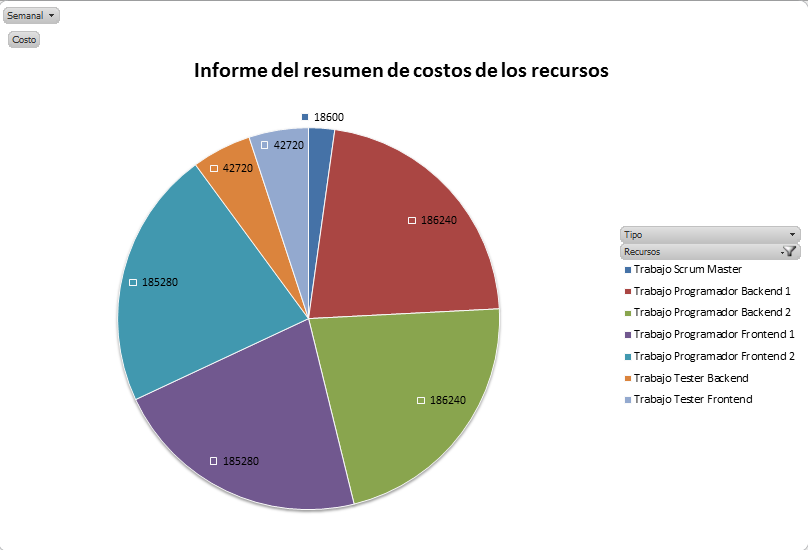
\includegraphics[width=\textwidth]{img/tp2_capitulo3/resumen-costos}
    \caption{Informe del resumen de costos de los recursos humanos.}
    \label{resumen-costos}
\end{figure}

\begin{comment}


PRECIOS BUSCADOS POR MI (IVÁN):
====================================
Oficina:
 $ 1.500 - 5 SECCION. SIN EXPENSAS.

Alquilo privado en lugar con 2 privados mas. Sin expensas. Excelente ubicación, servicio de wi-fi, calefacción, sala de reuniones, sala de espera/recepción, cocina, baño completo. Lugar en via publica para estacionar comodamente. Sistema de vigilancia monitoreada con alarma. Preferentemente para Arquitecto, Ingeniero, Agrimensor, Contador, Ingeniero

http://napsix.mdzol.com/mendoza/viewPost.jsp?id=c1650036-25ab-45c5-8d13-4f9510b3d6e0
====================================
Computadoras Notebooks:
Notebook DELL I3442/3_I541TBW8S_5 Intel Core i5

$13.399
Código: 211.147 

Generales

    Marca CPU Intel
    Versión CPU Core i5
    Modelo CPU 4210U
    Velocidad CPU 2.7 GHz
    Memoria Ram 4 GB
    Pad Numérico No
    Unidad Óptica DVD+/-RW
    Procesador Gráfico Intel® HD Graphics 4400
    Sistema Operativo Windows 8
    Versión OS 8.1
    WebCam Incorporada
    Capacidad Disco Rígido 1TB
    Color Negro
    Origen China

Pantalla

    Tamaño de Pantalla 14"
    Tipo de Pantalla LED
    Resolución 1366 x 768

Conectividad

    Wi-Fi Sí
    Bluetooth Sí
    Versión Bluetooth 4.0
    USB 2.0 2
    Puerto Ethernet No
    Salida HDMI No 
https://www.garbarino.com/producto/notebook-dell-i34423_i541tbw8s_5-intel-core-i5/a170746c2a
====================================
Sillas:
Silla Executive
Código 	A-1202
Alto 	116 cm
Ancho 	60 cm
Profundidad 	69 cm
Apilables 	NO
Colores Disponibles 	
$3100
http://desillas.com/producto-28-silla-de-oficina-y-computadora-con-ruedas-ergonomica-y-regulable.html
====================================
Sillon
Sillon Barcelona
Código 	F-1382
Alto 	75 cm
Ancho 	75 cm
Profundidad 	80 cm
Apilables 	NO
Colores Disponibles 	
$3900
http://desillas.com/producto-115-sillon-barcelona-cromado.html
====================================
Escritorio Para Oficina / Mesas Para Computacion
Para 1 persona - 120cm x 75 cm x 60 cm
Precio
$ 949.00	
http://articulo.mercadolibre.com.ar/MLA-562294620-escritorio-muebles-para-oficina-mesas-para-computacion-_JM

====================================
Database Server:
HP ProLiant DL980 G7 E7-2830 2.13GHz 8 Core 4p Server(AM449A) 
(AM449A)
$33,292.49*DOLARES

    Processor       Intel® Xeon® E7-2830 (8 core, 2.13 GHz, 24MB, 105W) 
    Number of processors            4
    Processor core available       8 
    Form factor (fully configured)        8U 
    Power supply type        (4) 1200W Platinum hot plug power supply kit Common Slot 
    Expansion slots
            (16) PCIe/PCIx
            For detail descriptions reference the QuickSpec
Memory
    Memory, standard        128GB (16x8GB) RDIMM 
    Memory slots        128 DIMM slots 
    Memory type            2R x4 PC3-10600R-9
Storage
    Included hard drives
        None ship standard; Supports up to (8) SFF SAS 
    Optical drive type
        Slim SATA DVD-RW 
Controller Cards
    Network controller
        1Gb NC375i Multifunction Ethernet Adapter 4 Ports per controller 
    Storage controller
        (1) Smart Array P410i/512MB FBWC 
Dimensions and weight
    Dimensions (W x D x H)
        35.02 x 43.99 x 69.59 cm (13.79 x 17.32 x 27.4 in) 
    Weight
        92.98 kg (205 lb) 
Server management
    Infrastructure management
        Lights-Out100 (Standard), HP Insight Control (Optional) 
http://www8.hp.com/us/en/products/proliant-servers/product-detail.html?oid=5099264#!tab=specs

======================================
web server:
 HP ProLiant DL300 Servers
HP ProLiant DL380 Gen9 E5-2690v3 2P 32GB-R P440ar 8SFF 2x10Gb 2x800W OneView Server(803861-B21)
$11,597.49*DOLARES
    Processor       Intel® Xeon® E5-2690 v3 (12 core, 2.6 GHz, 30MB, 135W) 
    Number of processors            2
    Processor core Available       12 
    Form factor (fully configured)        2U 
    Power supply type        (2) 800W Flex Slot Platinum hot plug power supply kit 
    Expansion slots  		(6) PCIe
Memory
    Memory, standard        32GB (2x16GB) RDIMM 
    Memory slots        24 DIMM slots 
    Memory type            2R x4 PC4-2133P-R
Storage
    Drive description
            ((4) or (12)) LFF SAS/SATA/SSD
            ((8) or (16) or (24)) SFF SAS/SATA/SSD
            (2) SFF Rear drive optional or
            (3) LFF Rear drive optional
            Hot plug, depending on model
    Included hard drives
        (8) SFF None ship standard; Supports up to (8) SFF SAS/SATA/SSD hot plug drives 
Controller Cards
    Network controller
        1Gb 331FLR Ethernet Adapter 4 Ports per controller; 10Gb 533FLR-T FlexFabric Adapter 2 Ports per controller 
    Storage controller
        (1) Smart Array P440ar/2GB FBWC 
Dimensions and weight
    Dimensons (W x D x H)        44.54 x 67.94 x 8.73 cm (17.54 x 26.75 x 3.44 in) 
    Weight        14.76 kg (minimum) (32.6 (minimum)) 
Server management
    Infrastructure management
        iLO Management (standard), Intelligent Provisioning (standard), HP OneView Advanced (standard) 
        
http://www8.hp.com/us/en/products/proliant-servers/product-detail.html?oid=7630563#!tab=specs

======================================
API SERVER:
 HP ProLiant DL300 Servers
HP ProLiant DL380 Gen9 E5-2690v3 2P 32GB-R P440ar 8SFF 2x10Gb 2x800W OneView Server(803861-B21)
$11,597.49* DOLARES

    Processor        Intel® Xeon® E5-2690 v3 (12 core, 2.6 GHz, 30MB, 135W) 
    Number of processors            2
    Processor core available        12 
    Form factor (fully configured)        2U 
    Power supply type        (2) 800W Flex Slot Platinum hot plug power supply kit 
    Expansion slots            (6) PCIe
Memory
    Memory, standard        32GB (2x16GB) RDIMM 
    Memory slots        24 DIMM slots 
    Memory type            2R x4 PC4-2133P-R
Storage
    Drive description
            ((4) or (12)) LFF SAS/SATA/SSD
            ((8) or (16) or (24)) SFF SAS/SATA/SSD
            (2) SFF Rear drive optional or
            (3) LFF Rear drive optional
            Hot plug, depending on model
    Included hard drives
        (8) SFF None ship standard; Supports up to (8) SFF SAS/SATA/SSD hot plug drives 
    Optical drive type
        Optional 
Controller Cards
    Network controller
        1Gb 331FLR Ethernet Adapter 4 Ports per controller; 10Gb 533FLR-T FlexFabric Adapter 2 Ports per controller 
    Storage controller        (1) Smart Array P440ar/2GB FBWC 
Dimensions and weight
    Dimensions (W x D x H)        44.54 x 67.94 x 8.73 cm (17.54 x 26.75 x 3.44 in) 
    Weight        14.76 kg (minimum) (32.6 (minimum)) 
Server management
    Infrastructure management
        iLO Management (standard), Intelligent Provisioning (standard), HP OneView Advanced (standard) 
        
http://www8.hp.com/us/en/products/proliant-servers/product-detail.html?oid=7630563#!tab=specs

==============================
Internet:

http://negocios.telefonica.com.ar/productos/telefonia/tenes-linea/banda-ancha-ip-fija/
\end{comment}


\section{Análisis de riesgos}

\subsection{Introducción}

\subsubsection{¿Qué es el análisis de riesgo?}

El análisis de riesgos es un proceso que comprende la identificación de elementos intervinientes en el proyecto, sus vulnerabilidades y amenazas a los que se encuentran expuestos, así como su probabilidad de ocurrencia y el impacto de las mismas, a fin de determinar los controles adecuados para aceptar, disminuir, transferir o evitar la ocurrencia del riesgo.

\subsubsection{¿Qué es un riesgo?}

Un riesgo de un proyecto es un evento o condición incierto que, si se produce, tendrá un efecto positivo o negativo sobre al menos un objetivo del proyecto, como tiempo, coste, alcance o calidad. El riesgo está compuesto de tres componentes esenciales, un evento definible, probabilidad de ocurrencia, consecuencia de la ocurrencia (impacto).

\subsubsection{Definición de términos}
% Clasificación de riesgos, internos, externos..
	\begin{itemize}
		\item \textbf{Activo}: Cualquier recurso, software, hardware, datos, administrativo, físico o persona.
        \item \textbf{Vulnerabilidad}: Debilidad que puede ser ``activada'' de forma accidental o intencionalmente.
        \item \textbf{Amenaza}: Representa la posibilidad de que se explote una vulnerabilidad de forma satisfactoria. Una fuente de amenazas no plantea un riesgo cuando no hay vulnerabilidades que puedan ser activadas.
        \item \textbf{Impacto}: Materialización de un riesgo; una medida del grado de daño o cambio sobre un activo.
        \item \textbf{Suposición}: Afirmación aceptada como real pero sin ningún tipo de prueba que la sustente.
	\end{itemize}
    
    \begin{comment}
		El riesgo está compuesto de tres componentes esenciales:
			- un evento definible
			- probabilidad de ocurrencia
			- consecuencia de la ocurrencia (impacto)
        
       RIESGOS
       el uso de nueva tecnología, o el aumento en la complejidad, rendimiento o agresividad en las fechas de entrega.
       pérdida de miembros clave en el equipo de trabajo, reorganización del negocio, u otros factores externos.

Riesgos de planificación/cronograma:

- Tareas con larga duración sin hitos bien definidos
- Tareas de camino crítico
- Tareas con múltiples predecesores
- Tareas estimadas de forma no realista
- Tareas dependientes de organizaciones externas
- Grandes hitos
- Cronograma sin suposiciones documentadas
- Restricciones de planificación
- Insuficiente información


Riesgos de recursos:
- Pérdida de contribuidores críticos
- Trabajo con proveedores no fiables
- Tareas no asignadas a nadie
- Formación
- Hardware y/o software


Riesgos financieros
- Desajustes en presupuesto
- Cambios en el coste de material

Riesgos de alcance y calidad
- Nueva tecnología no probada (incertidumbre)
- Cambios en los requisitos del cliente
- Herramientas no disponibles
- Alta tasa de defectos
- Alto impacto de negocio

Riesgos generales
- Mal entendimiento (requisitos, diseño...)
- Seguridad
- Pérdida de patrocinio
- Dificultades de lenguaje o comunicación
- Pérdida de información
        
        Tecnología nueva o no, disponibilidad de experiencia técnica, actuación del subcontratista, vendedor, personalización(riesgos de diseño), transición desde diseño a producción, disponibilidad de materiales.
        Prog. disponibilidad de recursos, planificación adecuada, restricción de programación, información insuficiente, dependencias de la empresa, dependencias del cliente
        Financiera. Fondos y presupuestos, exactitud de estimación, cambio en coste de material
        Contractual y legal. propiedad intelectual, políticas de gobierno, derechos de datos, ambiguedades de contacto, multas, derechos de patentes o incumplimientos
        
        http://www.brighthubpm.com/risk-management/88566-tool-for-assessing-project-risk/
        http://www.criptored.upm.es/intypedia/video.php?id=introduccion-gestion-riesgos&lang=es
        
    La velocidad del desarrollo tecnológico.
    Un retraso en el calendario acorta la ventana de la necesidad del proyecto que se esté desarrollando.
    La adaptabilidad del personal a nuevos lenguajes y metodologías.
    Clientes que invierten demasiado tiempo para exponer y dilatar sus requisitos.
    Fuga de conocimiento en el capital humano del proyecto.
    Proyectos pioneros tienen riesgos intensos en investigación, incluso puede que al borde de la I+D+i, con lo que un desarrollo de este tipo puede implicar en riesgos de presupuesto y adquisición de conocimiento.
	
    https://es.wikibooks.org/wiki/Direcci%C3%B3n_de_Proyectos/Planificaci%C3%B3n_de_los_riesgos_del_proyecto
	\end{comment}
    
\subsection{Riesgos detectados}
	\begin{enumerate}
\item \textbf{\textit{Abandono por parte de uno de los integrantes del grupo}}:

La posibilidad de que algún integrante abandone, ya sea por problemas de índole personal o laboral, en cierta medida es muy baja, pero si se concreta la repercusión en el grupo influirá de manera notable ya que en el equipo existe una planificación establecida con tareas y funciones previamente establecidas para desarrollar el proyecto. Algunas medidas que puedan llegar a evitar esto o disminuir el impacto, serían reuniones personales por parte del director con cada integrante de manera de detectar sus necesidades y brindarle diferentes soluciones, o al menos nos permitiría prever un posible abandono para salir a la búsqueda de un reemplazante e iniciar su capacitación para reemplazarlo.

\item \textbf{\textit{Falta de documentación de las tecnologías a utilizar}}:

Existe la posibilidad que la tecnología seleccionada no posea buena calidad de documentación (cuestiones sobre como resolver problemas o de como implementarla) y sea necesario hacer un análisis de las soluciones por nuestros propios medios. Esto provocaría atrasos en el desarrollo o en diferentes actividades del DevOps (Persona dedicada al desarrollo y despliegue de la infraestructura), corriendo el riesgo de no poder terminar con el proyecto a tiempo.

\item \textbf{\textit{Dificultad de aprendizaje de la tecnología a utilizar}}:

Los integrantes del proyecto tiene experiencia en programación pero para mejor el desarrollo se utilizarán herramientas nuevas que requerirán un período de adaptación a la misma, es por eso que se diagramó un plan de capacitación con cierta cantidad de horas cuyo principal riesgo es que no sea suficiente este tiempo para poder asimilar bien la tecnología y el conocimiento transmitido. Es posible que a algunos integrantes les sea suficiente pero hay una alta probabilidad de que no todos maduren el conocimiento de la misma manera como consecuencia de poseer diferentes capacidades de aprendizaje. Esto traería como consecuencia el atraso en el proyecto y horas sobrecargadas o un detrimento en la calidad del sistema a desarrollar. Algunas medidas preventivas podrían ser reunir al grupo y  elaborar un panorama con las diferentes dificultades a tener en cuenta de manera de sobrecargar con más horas a quien necesite más tiempo de capacitación. Otra forma de disminuir el impacto de dificultad de aprendizaje es realizar cursos que traten sobre las tecnologías a utilizar.

\item \textbf{\textit{Pérdida del soporte o compatibilidad hacia atrás de la tecnología que se está utilizando}}:

Suele suceder que ciertas tecnologías son actualizadas y deja de haber soporte para la versión que se está utilizando, esto produce, en el caso de los frameworks, que muchas  tareas que antes se realizaban automáticamente por el mismo, ahora necesiten mayor atención por parte del desarrollador. Otro caso se produce con las librerías que pierden soporte y produce que la aplicación se atrase con respecto a las tendencias y funciones mas utilizadas. Ambas situaciones provocan retrasos en el proyecto incrementando los costos. 

\item \textbf{\textit{Problemas de configuración de entornos de desarrollo y pruebas}}.

Es común que en la configuración de  entornos de desarrollo surjan problemas con las diferentes versiones y valores establecidos para dicha configuración. Se nos presenta como riesgo ya que es un tiempo considerable que se puede invertir en otra etapa y como se explicó en el riesgo anterior en el atraso de las tareas, se ve influenciado todo el proyecto, teniendo el riesgo de no llegar a tiempo con las entregas programadas. Una medida para evitar este problema sería encargar a cada uno de los miembros a aprender de fondo un tema y de este modo contar con una persona que comprenda el entorno de desarrollo y sea capaz de documentar en una ``wiki'' los pasos necesarios a seguir, para que todo el grupo sea capaz de llevarlo a cabo.

\item \textbf{\textit{Cambio de políticas o leyes gubernamentales}}:

El sistema se encuentra íntimamente relacionado con la información personal y por este motivo se encuentra sujeta a las modificaciones que hayan a nivel legal con respecto al manejo de datos personales. Actualmente  la Ley 26.529 establece los derechos del paciente referido a la documentación e información clínica y a la relación con los profesionales e instituciones de salud, si se produjera algún cambio sobre está ley nos afectaría directamente y tendríamos que re-analizar la situación.

Una medida a considerar puede ser mantener un acuerdo directo con el usuario, para que futuros cambios en el ámbito legal no nos afecte en forma directa.

\item \textbf{\textit{Aparición o detección de nuevos requerimientos}}:

Idealmente, luego de la etapa de Análisis, no deberían aparecer nuevos requerimientos. Sin embargo  la experiencia nos ha enseñado que no siempre es así. Este es un riesgo a tener en cuenta ya que si aparece un nuevo requerimiento en una etapa avanzada del proyecto es muy probable que se retrasen otras tareas o modifiquen ciertos elementos ya cerrados que se verán afectados por los mismos.

\item \textbf{\textit{Adelanto de la fecha de entrega}}:

Puede darse la situación de que sea necesario entregar el sistema antes de lo previsto por que surge alguna oferta importante de un cliente, lo que provocaría agilizar los tiempo, (contratando a mas personal y por ende aumentando los costos) o recortar funcionalidades.

\end{enumerate}
\begin{comment}
	\begin{enumerate}
		\item Baja de un integrante
        En cualquier instante del proyecto puede ocurrir que uno de los integrantes decida dar una paso al costado en el ciclo de vida del proyecto, las razones por las cuáles una persona puede tomar esta decisión suelen ser muy variadas y en los casos en los cuáles no tienen que ver con el proyecto son muy difíciles de gestionar y prevenir. La ocurrencia de esta amenaza produce un gran impacto en el proyecto ya que actualmente se usan muchas tecnólogías diferentes utilizadas en proyectos de sistemas de información. La baja no solo deja la vacante y la necesidad de incorporación de otra persona sino también será necesaria la inducción y capacitación para que pueda desempeñarse como lo requiere el proyecto, también debemos considerar que los tiempos para esta introducción suelen ser variables de acuerdo al avance y es muy probable que se plantea el interrogante si la incorporación de una persona para el reemplazo será correcto o introducirá mayores complicaciones y retrasos a los tiempos del proyecto.
        \item Problemas con respecto a capacidades técnicas y tecnológicas
        Los integrantes actuales del equipo no poseen suficiente experiencia en las técnologías utitlizadas así como tampoco de las técnicas y metodologías que se seguirán al desarrollar el proyecto, los conocimientos requeridos en cuánto a sistemas de información si estan bien respaldados por los estudios académicos que presentan los integrantes. Los integrantes del equipo que se incorporen posteriormente es posible que tampoco tengan experiencia en las tecnologías y metodologías usadas.
        \item Incumplimiento de tareas
        En todo momento las tareas necesarias para cumplir con las etapas serán planificadas y divididas de acuerdo a los tiempos de trabajo de los integrantes, puede ocurrir que por motivos personales
        \item Problemas ocasionadas por tareas DevOps
        \item Conflictos entre los integrantes
        \item Cambio en políticas de gobierno (si aplican HCE universal cagamos)
        \item Modificaciones en las leyes (por ejemplo leyes que le otorguen responsabilidad al desarrollador de un sistema de salud cada vez que se produce daño o injuria en los pacientes a consecuencia del uso del mismo) %fuente: SSTD
        \item Detección de nuevos requerimientos / mala interpretación de requerimientos
        \item Pérdida de datos por fallas en seguridad o errores por parte de los integrantes.
        \item Errores de diseño
        \item Subestimación de la complejidad (Fallar en los deadlines y en los costos. Perder credibilidad)
        \item Falta de claridad en roles y responsabilidades
        \item Falta de recursos para capacitación % aspectos organizacionales
	\end{enumerate}
    
    Posible riesgo, una vez implementado la probabilidad de que se filtro información sensible de una persona.
    
\end{comment}


\subsection{Análisis de riesgos}

El análisis de riesgos evalúa los riesgos identificados para determinar la probabilidad de que ocurran, el impacto del riesgo, el impacto acumulativo de múltiples riesgos y la prioridad de cada riesgo.

A continuación, se explicitan los pasos del análisis de riesgos y se detallan gráficamente.
Se define una tabla con los riesgos y sus probabilidades, que representa un análisis cuantitativo de los mismos.

\begin{enumerate}
	\item Determinación del criterio para evaluar la probabilidad.
    La tabla resultado de este paso puede observarse en el \textbf{Cuadro \ref{criterios-riesgos}}.
    
	\begin{table}[h]
        \centering
        \resizebox{\textwidth}{!}{
        \begin{tabular}{|c|c|c|}
            \hline
            \multicolumn{3}{|c|}{{\bf Tabla resumen de costos relevados}} \\ \hline
            {\bf Rango de probabilidad}  & {\bf Expresión del lenguaje natural} & {\bf Valor}  \\ \hline
            1-10\%                      & Baja                                 & 5\%                     \\ \hline
            11-25\%                     & Poco probable                        & 18\%                     \\ \hline
            26-55\%                     & Media                                & 40\%                     \\ \hline
            56-80\%                     & Altamente probable                   & 68\%                     \\ \hline
            81-99\%                     & Casi seguro                          & 90\%                     \\ \hline
        \end{tabular}
        }
        \caption{Criterios para el análisis cuantitativo de riesgos.}
        \label{criterios-riesgos}
    \end{table}
    
    \item Se definen las probabilidades de ocurrencia para los riesgos detectados.
    La tabla resultado de este paso puede observarse en el \textbf{Cuadro \ref{Ocurrencia-riesgo}}.
    
    \begin{table}[h]
        \centering
        \begin{tabulary}{\textwidth}{|L|C|C|}
            \hline
            %\multicolumn{3}{|C|}{{\bf Tabla de probabilidades de ocurrencia cuantificada}} \\ \hline
            {\bf Riesgo} & {\bf Expresión del lenguaje natural}        & {\bf Probabilidad de ocurrencia} \\ \hline
            Abandono por parte de uno de los integrantes del grupo                                                   & Baja & 5\% \\ \hline
            Falta de documentación de las tecnologías a utilizar                                                     & Media  & 40\% \\ \hline
            Dificultad de aprendizaje de la tecnología a utilizar                                                    & Media & 40\%   \\ \hline
            Pérdida del soporte o compatibilidad hacia atrás de la tecnología que se está utilizando & Poco probable & 18\%  \\ \hline
            Problemas de configuración de entornos de desarrollo y pruebas                                           & Media & 40\%  \\ \hline
            Cambio de políticas o leyes gubernamentales                                                              & Baja  & 5\%       \\ \hline
            Aparición o detección de nuevos requerimientos                                                           & Media  & 40\% \\ \hline
            Adelanto de la fecha de entrega                                                                          & Baja & 5\%  \\ \hline
                     
        \end{tabulary}
        \caption{Probabilidades de ocurrencia de riesgos.}
        \label{Ocurrencia-riesgo}
    \end{table}

	\item Se establece el criterio para evaluar el nivel de impacto calculado en semanas y meses.
    La tabla resultado de este paso puede observarse en el \textbf{Cuadro \ref{Criterio-impacto}}.
    
	\begin{table}[h]
        \centering
        \begin{tabular}{|c|c|c|}
            \hline
            \multicolumn{3}{|c|}{{\bf Tabla cuantificación del impacto}}          \\ \hline
            {\bf Criterio}      & {\bf Impacto}           & {\bf Valor}           \\ \hline
             Despreciable       & Menos de una semana     & 1                     \\ \hline
             Bajo               & Hasta dos semanas       & 2                     \\ \hline
             Medio              & Hasta 1 mes             & 3                     \\ \hline
             Alto               & Hasta 2 meses           & 4                     \\ \hline
             Crítico            & Más de 2 meses          & 5                     \\ \hline
        \end{tabular}
        \caption{Criterios de impacto}
        \label{Criterio-impacto}
    \end{table}
    
    \item Se define el impacto, suponiendo la ocurrencia de los riesgos.
    La tabla resultado de este paso puede observarse en el \textbf{Cuadro \ref{Riesgo-impacto}}.
    
    \begin{table}[h]
        \centering
        \begin{tabulary}{\textwidth}{|L|c|c|}
            \hline
            %\multicolumn{3}{|c|}{{\bf Tabla de ocurrencia de riesgos y su correspondiente impacto}}  \\ \hline
            {\bf Riesgo}      & {\bf Criterio}           & {\bf Valor}                               \\ \hline
             Abandono por parte de uno de los integrantes del grupo                                   & Medio   & 3 \\ \hline
             Falta de documentación de las tecnologías a utilizar                                     & Alto    & 4 \\ \hline
             Dificultad de aprendizaje de la tecnología a utilizar                                    & Medio   & 3 \\ \hline
             Pérdida del soporte o compatibilidad hacia atrás de la tecnología que se está utilizando & Alto    & 4  \\ \hline
             Problemas de configuración de entornos de desarrollo y pruebas                           & Bajo    & 2 \\ \hline
             Cambio de políticas o leyes gubernamentales                                              & Crítico & 5 \\ \hline
             Aparición o detección de nuevos requerimientos                                           & Medio   & 3 \\ \hline
             Adelanto de la fecha de entrega                                                          & Alto    & 4 \\ \hline
        \end{tabulary}
        \caption{Impacto sobre la ocurrencia de los riesgos}
        \label{Riesgo-impacto}
    \end{table}
    
    \item \textbf{Exposición al riesgo}:
    Teniendo en cuenta la probabilidad de ocurrencia y el impacto, se define la exposición al riesgo como el producto entre los mismos.
    
    \item Se establece el criterio para determinar la exposición al riesgo.
    La tabla resultado de este paso puede observarse en el \textbf{Cuadro \ref{Riesgo-exposicion}}.
    
    \begin{table}[h]
        \centering
        \begin{tabular}{|c|c|}
            \hline
            \multicolumn{2}{|c|}{{\bf Tabla de cuantificación de la exposición al riesgo}}  \\ \hline
            {\bf Criterio}      & {\bf Valor}                                               \\ \hline
             Baja      & Riesgo $\leq$ 1          \\ \hline
             Media     & 1 $<$ Riesgo $\leq$ 2    \\ \hline
             Alta      & 2 $<$ Riesgo $\leq$ 3    \\ \hline
             Muy alta  & 3 $<$ Riesgo             \\ \hline
        \end{tabular}
        \caption{Exposición al riesgo.}
        \label{Riesgo-exposicion}
    \end{table}
    
    \item Se define la tabla final de riesgos, probabilidad de ocurrencia, impacto y exposición al riesgo. 
    La tabla resultado de este último paso puede observarse en el \textbf{Cuadro \ref{Final-analisis-riesgo}}.
    
    \begin{table}[h]
        \centering
        \begin{tabulary}{\textwidth}{|L|C|c|c|c|}
            \hline
            %\multicolumn{5}{|c|}{{\bf Tabla final análisis de riesgo}}  \\ \hline
            {\bf Riesgo}      & {\bf Probabilidad de ocurrencia} & {\bf Impacto} & {\bf Exposición} & {\bf Criterio}    \\ \hline
             Abandono por parte de uno de los integrantes del grupo                                   & 5\%  & 3 & 0,15 & Baja \\ \hline
             Falta de documentación de las tecnologías a utilizar                                     & 40\% & 4 & 1,6 & Media \\ \hline
             Dificultad de aprendizaje de la tecnología a utilizar                                    & 40\% & 3 & 1,2 & Media \\ \hline
             Pérdida del soporte o compatibilidad hacia atrás de la tecnología que se está utilizando & 18\% & 4 & 0,72 & Baja \\ \hline
             Problemas de configuración de entornos de desarrollo y pruebas                           & 40\% & 2 & 0,8 & Baja \\ \hline
             Cambio de políticas o leyes gubernamentales                                              & 5\%  & 5 & 0,25 & Baja \\ \hline
             Aparición o detección de nuevos requerimientos                                           & 40\% & 3 & 1,2 & Media \\ \hline
             Adelanto de la fecha de entrega                                                          & 5\%  & 4 & 0,2 & Baja \\ \hline
        \end{tabulary}
        \caption{Análisis de riesgos.}
        \label{Final-analisis-riesgo}
    \end{table}
    
\end{enumerate}



\subsection{Acciones preventivas}

	\begin{enumerate}
		\item \textbf{\textit{Abandono por parte de uno de los integrantes del grupo}}
        	\begin{itemize}
				\item Si los motivos están relacionados con el proyecto el equipo puede detectar cuál es la fuente del problema y tratar de encontrar una solución para no perderlo.
                \item Firmar un contrato por el plazo que dura el proyecto o las etapas críticas para evitar la deserción en tiempos claves.
                \item Buscar formas de brindar motivaciones positivas que ayuden a hacer más fuerte el vínculo de la persona con el proyecto
			\end{itemize}
        \item \textbf{\textit{Falta de documentación de las tecnologías a utilizar}}
        	\begin{itemize}
				\item Realizar un relevamiento detallado de las tecnologías a utilizar, investigando la documentación online, foros de discusión orientado a la informática conocidos que debaten sobre la herramienta, listas de distribución de correo para así tomar una decisión con más información.
                \item Contacto con personas que conozcan la tecnología y nos brinden su tiempo para ayudarnos con los temas necesarios.
			\end{itemize}
        \item \textbf{\textit{Dificultad de aprendizaje de la tecnología a utilizar}}
        	\begin{itemize}
				\item Elegir una tecnología bien documentada,  de software libre, que garantice el mantenimiento gracias a la gran comunidad que lo respalda.
                \item Utilizar tecnologías robustas, basada en los conocimientos de los integrantes del equipo, usadas en herramientas y con mucho tiempo el mercado.
                \item Cursos web pueden ser una alternativa para la capacitación cuando no encontramos disponibilidad de profesionales en la zona en la que se desenvuelven los integrantes del proyecto.
                \item Reuniones continuas de los integrantes para evacuar y buscar soluciones a dudas en equipo.
			\end{itemize}
        \item \textbf{\textit{Pérdida del soporte o compatibilidad hacia atrás de la tecnología que se está utilizando}}
        	\begin{itemize}
				\item Investigación sobre la visión y objetivos de los frameworks que el equipo puede llegar a usar.
                \item Estudio de los intervalos de tiempo entre versionado para determinar la probabilidad de ocurrencia de una nueva versión de la tecnología durante el desarrollo del proyecto.
                \item Evaluación de casos anteriores de cambio de versión para determinar si la transición fue manejada de buena forma o surgieron muchas complicaciones.
			\end{itemize}
        \item \textbf{\textit{Problemas de configuración de entornos de desarrollo y pruebas}}
        	\begin{itemize}
				\item Planificar configuraciones con tiempo
                \item Buscar documentación actualizada.
                \item Probar previamente las configuraciones en un entorno de prueba, un entorno que no demande estabilidad.
                \item Consultar con expertos en el área.
			\end{itemize}
        \item \textbf{\textit{Cambio de políticas o leyes gubernamentales}}
        	\begin{itemize}
				\item Son muy difíciles de prevenir, lo que podríamos hacer es analizar que es lo que sucede en países que hace tiempo marcan las tendencias legales, tendencias que el país podría seguir y que podrían afectar al sistema.
                \item Contar con asesores que vislumbren posibles cambios en la legislación nacional e internacional, implementando reformas que alineen la visión del sistema con la del país en materia legal médica.
			\end{itemize}
        \item \textbf{\textit{Aparición o detección de nuevos requerimientos}}
        	\begin{itemize}
				\item Dedicar un tiempo adecuado al relevamiento.
                \item Selección de metodología que permita tener un feedback del cliente en un corto plazo.
                \item Buenas prácticas de diseño para desacoplar las funcionalidades y así lograr la máxima independencia entre ellas.
                \item Planificar márgenes de tiempo que nos permitan adaptar el sistema a estos nuevos requerimientos
			\end{itemize}
        \item \textbf{\textit{Adelanto de la fecha de entrega del sistema}}
        	\begin{itemize}
				\item Buena planificación, indicando los sprints correspondientes que se llevarían a cabo en cada fecha determinada, para de este modo poder ofrecer de forma correcta cuales son las funciones a entregar en cada una de las fecha correspondientes, siempre teniendo en cuenta la integridad del sistema.
			\end{itemize}
	\end{enumerate}

\begin{comment}
	Gestión de riesgos
    La gestión de riesgos se lleva a cabo:
- En la elaboración de una propuesta, cuando se planifica el proyecto
- A intervalos regulares durante la vida del proyecto: por ejemplo, como   parten  de los  informes de estado del proyecto.
- Cuando hay un cambio de alcance en el proyecto Por tanto, es un proceso   iterativo y recurrente a lo largo de toda la vida del proyecto.

- Se reduce los costes del proyecto
- Se mejora la satisfacción del cliente
- Se incrementa la capacidad y probabilidades de éxito
- Facilita el desarrollo del proyecto
- Disminuye drásticamente las sorpresas en los proyectos
- Ayuda a la empresa a conseguir los objetivos de negocio y proyecto evitando
  problemas que podrían causar pérdidas inesperadas y no planificadas
  
	Plan de gestión de riesgo
- Una estrategia de gestión de riesgos
- Alcance del esfuerzo en gestión de riesgos
- Cómo se piensa llevar a cabo la identificación de riesgos
- Cómo se va a llevar a cabo el análisis de riesgos (cualitativo, cuantitativo,  
  priorización)
- Cómo se va a llevar a cabo el plan de respuesta (no debe contener los
  propios   planes de respuesta ni tratar riesgos concretos)
- Cómo se va a llevar a cabo la monitorización y control
- Presupuesto de gestión de riesgos
- Calendario de actividades de gestión de riesgos
- Roles y responsabilidades

\end{comment}

\subsection{Acciones ante la ocurrencia de la amenaza}

	\begin{enumerate}
		\item \textbf{\textit{Abandono por parte de uno de los integrantes del grupo}}
        	\begin{itemize}
				\item Intentar convencer a la persona que deponga su decisión por distintos medios, que tengan que ver con el motivo del abandono.
                \item Si se produce el abandono, se podrían redistribuir las tareas que tenía el integrante para amortiguar el impacto en la transición hasta incorporar un reemplazante.
                \item Tener preparado el perfil que ocupa el integrante para iniciar el proceso de reclutamiento.
			\end{itemize}
        \item \textbf{\textit{Falta de documentación de las tecnologías a utilizar}}
        	\begin{itemize}
				\item Recurrir a otros medios, contactar participantes de foros que utilicen la tecnología.              
			\end{itemize}
        \item \textbf{\textit{Dificultad de aprendizaje de la tecnología a utilizar}}
        	\begin{itemize}
				\item Consultar otras fuentes de información.
                \item Reuniones de capacitación dinámica entre los mismos participantes.
			\end{itemize}
        \item \textbf{\textit{Pérdida del soporte o compatibilidad hacia atrás de la tecnología que se está utilizando}}
        	\begin{itemize}
				\item Cambio de la tecnología, representa el cambio más radical y la última opción a elegir pero es una opción al fin cuando la situación es muy compleja.
                \item Verificar el tiempo que tendrá soporte la tecnología usada para planificar y gestionar las tareas de migración.
			\end{itemize}
        \item \textbf{\textit{Problemas de configuración de entornos de desarrollo y pruebas}}
        	\begin{itemize}
				\item Cambiar de entorno, versión, herramienta.
                \item Consultar a un experto
                \item Evaluar la posibilidad de prescindir de la herramienta.
			\end{itemize}
        \item \textbf{\textit{Cambio de políticas o leyes gubernamentales}}
        	\begin{itemize}
				\item Adaptar el sistema a las nuevas leyes.
			\end{itemize}
        \item \textbf{\textit{Aparición o detección de nuevos requerimientos}}
        	\begin{itemize}
				\item Incorporar personal que se encargue de estos nuevos requerimientos.
                \item Planificar nuevos sprints o replanificar los existentes para atender el o los requerimientos.              
			\end{itemize}
        \item \textbf{\textit{Adelanto de la fecha de entrega del sistema}}
        	\begin{itemize}
				\item Evaluar la posibilidad de incorporar personal siempre y cuando su incorporación no provoque retrasos y si una mejora real.
                \item Planificar horas extras de los participantes con sus correspondientes recompensas y retribuciones para mantener un buen ambiente en el equipo.
			\end{itemize}
	\end{enumerate}
    
\begin{comment}
Cuantificar riesgos, analizar resultados

− Identificar todos los riesgos conocidos del proyecto
− Realizar una evaluación de la probabilidad de ocurrencia y del impacto
    potencial
− Cuantificar cual sería el coste de los riesgos en caso de que ocurrieran
− Crear planes de acción para gestionar los riesgos de alta prioridad
− Reconocer y gestionar los riesgos lo antes posible
\end{comment}


\section{Análisis de impacto ambiental}


\subsection{Introducción}
	El \textbf{análisis de impacto ambiental} es un procedimiento técnico-administrativo que sirve para identificar, prevenir e interpretar los impactos ambientales que producirá un proyecto en su entorno, en caso de ser ejecutado, todo ello con el fin de que la administración competente pueda aceptarlo, rechazarlo o modificarlo.
    
    El proyecto impacta directamente en la forma en que la persona gestiona su información de salud, por lo que es sumamente importante que se conozca sus hábitos y opiniones respecto a los sistemas de información.
    Un estudio realizado en Estados Unidos, conducido por Harris Interactive, encontró que la opinión pública está dividida sobre si el beneficio supera los riesgos o no, para la utilización de un registro médico electrónico (\textbf{47\%} a favor versus \textbf{48\%} en contra).
    
    Por otro lado, un estudio realizado por una importante institución médica del país reveló que el \textbf{82\%} de personas encuestadas querrían disponer de herramientas para rastrear su propia información en salud y asegurar su derecho a la privacidad.
    
    En el \textbf{Cuadro \ref{Preocupacion-seguridad}} se puede observar cómo respondieron los encuestados en estos aspectos relacionados a la seguridad y privacidad de su información médica.
    
    \begin{table}[h]
        \centering
        \begin{tabulary}{\textwidth}{|L|C|C|C|C|}
            \hline
            %\multicolumn{5}{|c|}{{\bf Preocupación sobre seguridad y privacidad de la información médica}}  \\ \hline
             & {\bf Muy preocupado} & {\bf Algo preocupado} &{\bf No muy preocupado} &{\bf Nada preocupado} \\ \hline
             \textbf{Información personal sensible relacionada con la salud puede difundirse por una seguridad débil}               & 38 & 32 & 16 & 13 \\ \hline
             \textbf{Se puede compartir información médica sin su consentimiento}                                                   & 42 & 27 & 18 & 13 \\ \hline
             \textbf{La seguridad del nuevo sistema no va a ser suficiente}                                                         & 34 & 35 & 18 & 12 \\ \hline
             \textbf{Algunas personas no van a revelar información sensible por miedo a que se almacenen en el sistema informático} & 29 & 36 & 20 & 13 \\ \hline
             \textbf{La informatización puede aumentar en lugar de disminuir los errores médicos}                                   & 29 & 36 & 22 & 13 \\ \hline
        \end{tabulary}
        \caption{Preocupación sobre seguridad y privacidad de la información médica.}
        \label{Preocupacion-seguridad}
    \end{table}
    
    Puede decirse entonces que garantizar la privacidad y la confidencialidad beneficia también al sistema de salud, ya que un paciente que sabe que su información clínica no será accedida de forma inapropiada, se sentirá más cómodo a la hora de revelarla y lograr esta confianza es vital para mantener la relación sistema-paciente.

	\subsection{Impacto en el medio ambiente}

Es  posible interpretar por  \textbf{impacto  ambiental} a las alteraciones  que  la  construcción  y operación (o sea, de realizar una actividad) de un proyecto de desarrollo introducen en el medio, y las formas de evitarlas o minimizarlas, entendiendo esta diferencia de cómo quedaría el ambiente con y sin el proyecto.
Es decir, cómo hubiera evolucionado sin el proyecto.

{\correccionTexto
La alteración que se produce en el ambiente cuando se lleva a cabo un proyecto o una actividad no siempre es negativa.
Puede ser favorable o desfavorable para el medio. 
}

	\subsubsection{Expresión técnica del impacto ambiental}

Desde la óptica técnica, el impacto ambiental tiene su origen en una causa, que puede ser en nuestro caso un proyecto de desarrollo, la cual crea perturbaciones (alteraciones) positivas o negativas en los  elementos  medioambientales, y cuyo impacto se comprende mediante la  valoración  de  la afectación. 
 
Esta alteración se cualifica y cuantifica en el área de influencia donde se desarrolle el proyecto, sobre: la función ecológica que cumplen los elementos naturales y percepción del paisaje, 
las infraestructuras, las estructuras civiles y el uso/ocupación del territorio, los elementos de los componentes de las dimensiones económica y social, y los rasgos y patrimonio cultural de la población humana asentada en el lugar.

	\subsubsection{Tipos de impacto ambiental}
 
Existen diferentes tipos de impacto ambiental, y en la práctica un mismo impacto puede ser catalogado en diferentes clases o categorías de impacto.
A continuación, se dan a conocer algunas de estas clases. Se pueden clasificar por variación de la calidad ambiental, por el grado de  destrucción, por la extensión,  por  el  momento  de  manifestarse,  por  su  persistencia,  por  su capacidad  de  recuperación,  por  la  relación  causa–efecto,  por  la  interrelación  de  acciones,  por  su periodicidad y por la necesidad de aplicación de medidas correctoras. 
 
 
De importancia para este documento, y como se puede observar posteriormente al identificar y cuantificar impactos, son relevantes por variación de calidad del entorno los impactos positivos y negativos,  por  su  mejoramiento  o  desmejoramiento  de  la  calidad  ambiental  en  el  área  de influencia.
Así mismo, se tendrán en cuenta por intensidad los impactos muy alto, alto, medio y bajo; y, por su capacidad de recuperación, los impactos reversibles, irreversibles, recuperables, mitigables e irrecuperables.  

De estos últimos, es reversible cuando la naturaleza asimila la alteración y por si misma torna a su  calidad  ambiental, e irreversible cuando el medio  ambiente  no  asimila  la alteración  y  la calidad ambiental  no  vuelve  por  mecanismos  propios  de  lo  natural,  a  niveles  que  poseía  antes  de  la actuación. 
 
Cuando  se  aplican  medidas  correctoras  por  el  hombre,  el  impacto  se  reconoce  como recuperable cuando la perturbación puede eliminarse; mitigable al disminuirse de manera apreciable la alteración, e irrecuperable cuando la alteración o daño del entorno no se puede reparar.


{\correccionTexto
\subsubsection{Situación actual y el proyecto}

\begin{itemize}
    
    \item \textbf{Recursos naturales}:
    Los \textbf{resultados de análisis médicos} actualmente se imprimen en papel.
    De esta manera, no sólo se aumenta el consumo de este recurso, sino también el uso de productos de oficina como tinta o tóner.
    
    El proyecto propuesto produce una disminución en el uso de estos recursos, ya que fue planteado, desde la concepción, para ser una plataforma donde se dé soporte a la gestión de documentos asociados a la salud, y de esta forma prescindir de cualquier otro medio diferente al digital.
    Es importante recordar que los centros de análisis médicos tendrán la posibilidad de enviar directamente los resultados de análisis al paciente, a través de la API del sistema.

    La fabricación de papel no sólo afecta los costos de las empresas que imprimen los análisis, sino que también está relacionada con la contaminación acuífera (el agua utilizada en el proceso de procesar la celulosa generalmente es mezclada con solvente para darle el color blanco), la liberación de dióxido de carbono al aire y la deforestación (la cual tiene una incidencia directa en el efecto invernadero y el cambio climático, además del saneamiento del aire).

    \item \textbf{Diagnósticos por imágenes}:
    En cuanto a este tema, se presentan varias problemáticas a atender actualmente.
    
    El primero es la repetición de exámenes por pérdidas de placas, situación muy común actualmente a pesar de que hoy en día los estudios son entregados en un formato digital.
    Por otro lado, se observa un aumento de radiación ionizante a la persona, consecuencia directa de la pérdida de los estudios realizados previamente, lo que afecta negativamente su salud.
    
    Con el uso del sistema, el flujo de trabajo sería más eficiente, logrando los siguientes beneficios:
    
    \begin{itemize}
        \item Se disminuiría el tiempo en la atención médica ligada a radiología por el rápido acceso de los médicos a las imágenes.
        El acceso a la imagen correcta en el punto de atención sería una constante.
        
        \item Se visualizarían todas las imágenes históricas tomadas al paciente.
        
        \item Aumentaría el ahorro de costos potenciales, ya que no se imprimirían placas.
        
        \item Se evitaría la pérdida de placas.
        
        \item Disminuirían las repeticiones y la exposición repetida a los rayos X, por parte de los pacientes.
    \end{itemize}
    
    
    \item \textbf{Obsolescencia de dispositivos}:
    Es conocido que la industria electrónica es la que mayor daño hace al medio ambiente, no solo en forma directa (a través de su producción), sino también a través de los insumos que utiliza (minerales y metales pesados) y de los residuos generados.
    
    El contar con un sistema de carpeta digital de salud personal tiene por requisito fundamental el uso de estos dispositivos electrónicos, por parte tanto de pacientes como de médicos e instituciones de salud.
    Debido al alto grado de actualización e innovación tecnológica a nivel mundial, y teniendo en cuenta que los sistemas actuales deben adaptarse a este progreso tecnológico para aprovechar sus beneficios y los descubrimientos de que se vale, el sistema se basa en la tecnología y su avance constante para cumplir, de la mejor manera posible, con los objetivos con que fue concebido.
    
    
    \item \textbf{Contaminación vehicular}:
    Los automotores representan una fuente importante de contaminación del aire.
    La contaminación vehicular del aire produce efectos nocivos para la salud humana.
    Los estudios epidemiológicos demuestran que el aumento de los casos de enfermedades respiratorias está relacionado con las áreas urbanas, que poseen un elevado nivel de contaminación, a comparación de las áreas rurales.
    
    La implantación del sistema y uso por parte de la sociedad implicaría una menor concurrencia a hospitales e instituciones de salud, considerando aquellas asistencias que tengan por propósito el retiro de estudios médicos, consultas de baja complejidad o entrega de resultados médicos al profesional que los requirió, para su lectura y análisis.
    Esto tiene por consecuencia principal una menor cantidad de personas trasladándose a las instituciones de salud, lo que provoca reducir el parque automotor activo y, por lo tanto, eliminar una fracción de la contaminación vehicular existente en la actualidad.
    
    
    \item \textbf{Compartición inapropiada de datos}:
    La prioridad del sistema es la privacidad y completa confidencialidad de los datos médicos e información de salud de los usuarios.
    
    Sin embargo, y a pesar de todas las medidas de seguridad existentes y puestas a disposición del usuario, es éste quien decide qué aspectos de su información privada de salud compartir y a quién.
    El proveer al mismo de un sistema que gestiona toda esta información también le confiere el poder de, haciendo uso de una única herramienta, publicar la misma para que sea visible por quienes el considere oportuno.
    
    Es importante recalcar que el dueño de la información es el usuario, pero aún así es responsabilidad del sistema contar con el mayor nivel de transparencia y claridad al momento de ofrecer la compartición de datos, con el fin de que el mismo cuente con esta información y se responsabilice por las decisiones tomadas.
\end{itemize}


\subsubsection{Medición del impacto ambiental}

El método para realizar la medición del impacto ambiental incluye los siguientes factores:

\begin{itemize}
    \item \textbf{Signo}:
    Si es \textit{positivo} y sirve para mejorar el medio ambiente, o si es \textit{negativo} y degrada el medioambiente.
    
    \item \textbf{Magnitud}:
    Según la destrucción o cooperación con el ambiente, sea \textit{alta}, \textit{media} o \textit{baja}.
    
    \item \textbf{Alcance}:
    Según afecte a un lugar muy concreto (\textit{restringido}), a una zona algo mayor (\textit{local}), o a la totalidad del medio (\textit{global}).
    
    \item \textbf{Persistencia}:
    Se dice que es fugaz (\textit{baja}) si dura menos de 1 año; si dura de 1 a 3 años es temporal (\textit{media}) y pertinaz (\textit{alta}) si dura de 4 a diez años.
    Si es para siempre sería permanente.
\end{itemize}


La escala a utilizar será la siguiente:
\begin{itemize}
    \item \textbf{Magnitud}:
        \begin{itemize}
            \item Alta: 3 puntos.
            \item Media: 2 puntos.
            \item Baja: 1 punto.
        \end{itemize}
    
    \item \textbf{Alcance}:
        \begin{itemize}
            \item Global: 3 puntos.
            \item Local: 2 puntos.
            \item Restringido: 1 punto.
        \end{itemize}
    
    \item \textbf{Persistencia}:
        \begin{itemize}
            \item Alta: 3 puntos.
            \item Media: 2 puntos.
            \item Baja: 1 punto.
        \end{itemize}
\end{itemize}

En el caso del factor \textbf{Signo}, se utilizarán los valores \textit{$+$} (positivo) y \textit{$-$} (negativo).

En el \textbf{Cuadro \ref{evaluacion-impacto-ambiental}} se puede observar la evaluación del impacto ambiental, de los componentes ambientales especificados anteriormente, y utilizando los factores de evaluación descriptos.

\begin{table}[h]
    \centering
    \resizebox{\textwidth}{!}{%
        {\correccionTexto
        \begin{tabular}{|l|c|c|c|c|}
            
            \hline
            {\bf Componente ambiental} & {\bf Signo} & {\bf Magnitud} & {\bf Alcance} & {\bf Persistencia} \\ \hline
            {\bf Recursos naturales}
                                       & +           & Alta           & Global        & Alta               \\ \hline
            {\bf Diagnósticos por imágenes}
                                       & +           & Alta           & Global        & Alta               \\ \hline
            {\bf Obsolescencia de dispositivos}
                                       & -           & Baja           & Global        & Media              \\ \hline
            {\bf Contaminación vehicular}
                                       & +           & Media          & Global        & Alta               \\ \hline
            {\bf Compartición inapropiada de datos}
                                       & -           & Media          & Global        & Baja               \\ \hline
        \end{tabular}
        }
    }
    \caption{Evaluación del impacto ambiental.}
    \label{evaluacion-impacto-ambiental}
\end{table}
}

{\correccionTexto
Luego, por cada componente ambiental, se evalúa su puntaje, haciendo uso de la siguiente ponderación de los factores:

\begin{itemize}
    \item Magnitud: 40\%.
    \item Alcance: 40\%.
    \item Persistencia: 20\%.
\end{itemize}

Considerando, además, el signo de cada componente, sus respectivas puntuaciones se calculan a continuación:

\begin{itemize}
    \item \textbf{Recursos naturales}: $+ (3 \cdot 0.4 + 3 \cdot 0.4 + 3 \cdot 0.2) = 3$
    \item \textbf{Diagnósticos por imágenes}: $+ (3 \cdot 0.4 + 3 \cdot 0.4 + 3 \cdot 0.2) = 3$
    \item \textbf{Obsolescencia de dispositivos}: $- (1 \cdot 0.4 + 3 \cdot 0.4 + 2 \cdot 0.2) = -2$
    \item \textbf{Contaminación vehicular}: $+ (2 \cdot 0.4 + 3 \cdot 0.4 + 3 \cdot 0.2) = 2.6$
    \item \textbf{Compartición inapropiada de datos}: $- (2 \cdot 0.4 + 3 \cdot 0.4 + 1 \cdot 0.2) = -2.2$
\end{itemize}

Por lo tanto, el cálculo final se realiza mediante la suma de los diferentes componentes ambientales.
Si el resultado es positivo, indica que el impacto ambiental del proyecto es positivo.
De lo contrario, es negativo.

$3 + 3 - 2 + 2.6 - 2.2 = $ \textbf{$4.4$}

Como se puede observar, el resultado obtenido es \textbf{positivo}, con un valor de \textbf{4,4} puntos.
}

%IVAN CONDUCTOR DEL CAMION DE TERRABUSI NO ESCRIBAS ACA

\subsection{Conclusión}
{\correccionTexto
	Teniendo en cuenta los puntos mencionados anteriormente y la evaluación asociada a los mismos, se concluye que \textbf{el proyecto tendrá un impacto positivo sobre el ambiente} en el cual será introducido, ya que hace el trabajo más eficiente al poner a disposición del médico, en forma inmediata, toda la información necesaria para su trabajo.
}

    Además, su uso implica en forma directa la reducción de estudios repetidos por pérdida, la reducción de entrega de diagnósticos o resultados de análisis en papel, y la disminución de exposición de la persona a radiación.
    
    Por otro lado, se debe tener una especial consideración hacia el rechazo que aún genera el uso de sistemas de información para almacenar información delicada, y la preocupación por que estos datos sean manipulados por una persona no autorizada.
    
    Al trabajar profundamente sobre este aspecto de seguridad, y debido a que los demás aspectos anteriormente descritos son consecuencias directas del uso del sistema, se tendrá garantizada una \textbf{factibilidad completamente positiva en cuanto a impacto ambiental}.


